%%{ DOC HEAD

\pdfoutput=1
\documentclass[a4paper,11pt,titlepage,twoside]{book}

\usepackage[english]{babel}
\usepackage[utf8]{inputenc}
\usepackage{amssymb,amsmath}
\usepackage{algorithm,algpseudocode}
\usepackage[title,titletoc]{appendix}
\usepackage{latexsym}
\usepackage{a4wide}
\usepackage{color}
\usepackage{indentfirst}
\usepackage{graphicx}       %%% graphics for dvips
\usepackage{fancyhdr,lastpage}
\usepackage{longtable}
\usepackage{pifont}
\usepackage{makeidx}
\usepackage{multirow}
\usepackage{dcolumn}
\usepackage{epstopdf}
\usepackage{url}
\usepackage{listings}
\usepackage{relsize}
\usepackage{pdfpages}
\usepackage{url}
\usepackage{lipsum}
\usepackage{isotope}
\usepackage{verbatim}
\usepackage{xcolor}
\usepackage{tcolorbox}
\usepackage{subfig} % subfloat
\usepackage[export]{adjustbox}
\usepackage{tikz}

\usetikzlibrary{shapes.arrows,backgrounds,arrows,automata,shapes,positioning,calc,through}

%%{ ARROWS

\tikzset{
  myarrow/.style={
    draw,
    fill=orange,
    single arrow,
    minimum height=3.5ex,
    single arrow head extend=1ex
  }
}

\newcommand{\arrowup}{%
  \vspace{-0.8em}
  \tikz [baseline=-0.5ex]{\node [myarrow,rotate=90] {};}
  \vspace{-1.4em}
}

\newcommand{\arrowdown}{%
  \vspace{-0.8em}
  \tikz [baseline=-1ex]{\node [myarrow,rotate=-90] {};}
  \vspace{-1.5em}
}

\newcommand{\arrowright}{%
  \tikz [baseline=-1ex]{\node [myarrow,rotate=0] {};}
}

\newcommand{\arrowleft}{%
  \tikz [baseline=-1ex]{\node [myarrow,rotate=180] {};}
}

%%}

%%{ CHECKMARK

\def\checkmark{\tikz\fill[scale=0.4](0,.35) -- (.25,0) -- (1,.7) -- (.25,.15) -- cycle;}

%%}

\pgfdeclarelayer{background}
\pgfdeclarelayer{foreground}
\pgfsetlayers{background,main,foreground}

\tikzset{
  state/.style={
    rectangle,
    draw=black, very thick,
    minimum height=1.0em,
    text centered,
  },
  state_gray/.style={
    rectangle,
    draw=black, very thick,
    fill=gray!40,
    minimum height=1.0em,
    text centered,
  },
  state_white/.style={
    rectangle,
    draw=black, very thick,
    fill=white,
    minimum height=1.0em,
    text centered,
    text=black,
  },
  state_green/.style={
    rectangle,
    draw=black, very thick,
    fill=green!50,
    minimum height=1.0em,
    text centered,
    text=black,
  },
  state_red/.style={
    rectangle,
    draw=black, very thick,
    fill=red!70,
    minimum height=1.0em,
    text centered,
    text=black,
  },
  state_blue/.style={
    rectangle,
    draw=black, very thick,
    fill=blue!40,
    minimum height=1.0em,
    text centered,
    text=black,
  },
  final_state/.style={
    rectangle,
    rounded corners,
    draw=black, very thick,
    minimum height=2em,
    text centered,
  },
  initial_state/.style={
    rectangle,
    double=white,
    double distance=1pt,
    inner sep=2pt,
    draw=black, very thick,
    minimum height=2em,
    text centered,
  },
  point/.style={
    circle,
    inner sep=0pt,
    minimum size=3pt,
    fill=red
  },
}



% \newcommand{\includepaper}[1]{\includepdf[scale=0.85,pages=-,pagecommand={\thispagestyle{plain}}]{./papers_to_include_pdf/#1}}
% \newcommand{\includepaper}[1]{\conditionalClearPage \fullciteinbox{#1}{Here will be the pdf of the paper}}
\newcommand{\includepaper}[1]{\fullciteinbox{#1}{Here will be the pdf of the paper}}

%%{ fullcite box

\definecolor{light-gray}{gray}{0.95}
\newcommand{\fullciteinbox}[2]{%

\DeclareCiteCommand{\fullcite}
{\usebibmacro{prenote}}
{\clearfield{addendum}%
  \usedriver
  {\defcounter{minnames}{6}%
  \defcounter{maxnames}{6}}
{\thefield{entrytype}}}
{\multicitedelim}
{\usebibmacro{postnote}}

%\vspace{3em}%
%\raisebox{3em}[3em][3em]{%
% \vspace{-0.2em}
\begin{tcolorbox}[width=\textwidth,colback={light-gray},title={}]%
\ifx&#2&
\else
  \textbf{#2}:\\\\
\fi
\begin{minipage}[t]{0.07\linewidth}%
\raggedright%
\cite{#1}%
\end{minipage}%
\begin{minipage}[t]{0.93\linewidth}%
\fullcite{#1}%
\end{minipage}%
\end{tcolorbox}%
%}%
% \vspace{-0.5em}
}%

%%}

%%{ acronym

\usepackage[nolist,nohyperlinks]{acronym}
\acrodef{GPS}[GPS]{Global Positioning System}
\acrodef{SLAM}[SLAM]{Simultaneous Localization And Mapping}
\acrodef{SLAMs}[SLAMs]{Simultaneous Localization And Mapping systems}
\acrodef{GPS}[GPS]{Global Positioning System}
\acrodef{RTK}[RTK]{Real-time Kinematics}
\acrodef{GNSS}[GNSS]{Global Navigation Satellite System}
\acrodef{ROS}[ROS]{Robot Operating System}
\acrodef{API}[API]{Application Programming Interface}
\acrodef{UAV}[UAV]{Unmanned Aerial Vehicle}
\acrodef{UGV}[UGV]{Unmanned Ground Vehicle}
\acrodef{UV}[UV]{Ultra-Violet}
\acrodef{LED}[LED]{Light-emitting Diode}
\acrodef{MBZIRC}[MBZIRC]{Mohamed Bin Zayed International Robotics Challenge}
\acrodef{DARPA}[DARPA]{Defense Advanced Research Projects Agency}
\acrodef{IMU}[IMU]{Inertial Measurement Unit}
\acrodef{LTI}[LTI]{Linear time-invariant}
\acrodef{MPC}[MPC]{Model Predictive Control}
\acrodef{UVDAR}[UVDAR]{Ultra-Violet Direction And Ranging}
\acrodef{DOF}[DOF]{degree-of-freedom}
\acrodef{DOFs}[DOFs]{degrees-of-freedom}
\acrodef{LiDAR}[LiDAR]{Light Detection and Ranging}
\acrodef{ESC}[ESC]{Electronic Speed Controller}
\acrodef{LKF}[LKF]{Linear Kalman Filter}
\acrodef{UKF}[UKF]{Unscented Kalman Filter}
\acrodef{EKF}[EKF]{Extended Kalman Filter}
\acrodef{RAS}[RAS]{Robotics and Automation Society}
\acrodef{IEEE}[IEEE]{Institute of Electrical and Electronics Engineers}
\acrodef{MRS}[MRS]{Multi-robot Systems Group}

%%}


% change formatting of lists
\usepackage{enumitem}
\setlist{nosep}
% \setlist{noitemsep}
% how to format particular lists?
% \begin{itemize}[topsep=8pt,itemsep=4pt,partopsep=4pt, parsep=4pt]

% change spacing of the table of contents
% \usepackage{tocloft}
% \renewcommand\cftchapafterpnum{\vskip5pt}
% \renewcommand\cftsecafterpnum{\vskip5pt}

% change formatting of a chapter
\usepackage{titlesec}
\titleformat{\chapter}[block]
{\normalfont\huge\bfseries}{Chapter \thechapter\\\vspace{0.1em}\\}{1em}{\Huge}
% {?}{before}{after}
\titlespacing*{\chapter}{0pt}{-1em}{2em}

\hyphenation{Imaging}

%%{ BIBLATEX

\usepackage[backend=bibtex,defernumbers=true,style=ieee,sorting=ydnt,sortcites=true]{biblatex}

\renewcommand*{\bibfont}{\Font}

% \newcounter{mycounter}
% \setcounter{mycounter}{0}
% \newcounter{unrelatedcount}
% \setcounter{unrelatedcount}{0}
% \newcounter{totalcounter}
% \setcounter{totalcounter}{0}

% % Print labelnumbers with suffixes, adjust secondary labelnumber 1/2 (start new numbering of my publications)
% \makeatletter
% \AtDataInput{%
%   \ifkeyword{mine}
%   {
%     \addtocounter{mycounter}{1}
%   }
%   {}
%   \addtocounter{totalcounter}{1}
% }
% \makeatother

% Print labelnumbers with suffixes, adjust secondary labelnumber 2/2
\DeclareFieldFormat{labelnumber}{%
  \ifkeyword{mine}
  {\ifkeyword{phd_unrelated}
    {{\number\numexpr#1}a}%
{{\number\numexpr#1}a}}{#1}}

% {{\number\numexpr#1-\value{bbx:primcount}}a}

\addbibresource{main.bib}

\defbibenvironment{favoritebib}
{\itemize}
{\enditemize}
{\item}

%%}

%%{ CUSTOM MACROS

%%%%%%%%%%%%%%% changemargin environment begin %%%%%%%%%%%%%%%%%%%%%%%%%
\def\changemargin#1#2{\list{}{\rightmargin#2\leftmargin#1}\item[]}
\let\endchangemargin=\endlist
%%%%%%%%%%%%%%% changemargin environment end %%%%%%%%%%%%%%%%%%%%%%%%%

\newcommand{\strong}[1]{\textbf{#1}}
\newcommand{\coord}[1]{\textbf{#1}}
\newcommand{\norm}[1]{\left\lvert#1\right\rvert}
\newcommand{\m}[1]{\ensuremath{\mathbf{#1}}}
\newcommand\numberthis{\addtocounter{equation}{1}\tag{\theequation}}
\newcommand{\corrected}[1]{{\color{black} {#1}}}
% \newcommand{\comment}[1]{{\color{blue} {#1}}}
\newcommand{\add}[1]{{\color{green} {#1}}}
\newcommand{\todo}[1]{{\color{red} TODO {#1}}}
\newcommand{\updated}[1]{{\color{blue} {#1}}}
\newcommand{\reffig}[1]{Fig.~\ref{#1}}
\newcommand{\refalg}[1]{Alg.~\ref{#1}}
\newcommand{\refsec}[1]{Sec.~\ref{#1}}
\newcommand{\reftab}[1]{Table~\ref{#1}}
\newcommand{\real}{\mathbb{R}}
\newcommand{\red}[1]{{\color{red} #1}}
\newcommand{\minus}{\scalebox{0.75}[1.0]{$-$}}
\newcommand{\plus}{\scalebox{0.8}[0.8]{$+$}}
\newcommand{\figvspace}{\vspace{-1em}} % this may eventually do something, so far just a placeholder

\newcommand{\chapternoclear}[1]{
  \begingroup
  \let\cleardoublepage\clearpage
  \chapter{#1}
  \endgroup
}

\newcommand{\conditionalClearPage}{
  \ifdefined\printversion
  %\newpage{}
  %\thispagestyle{empty}
  \clearemptydoublepage
  %\cleardoublepage{\thispagestyle{empty}}
  \else
  \newpage{}
  \clearpage
  \fi
}

%%}

\newcommand{\Author}{Ing. Tomáš Báča}
\newcommand{\Supervisor}{Ing. Martin Saska, Dr. rer. nat.}
\newcommand{\SupervisorSpecialist}{Ing. Michal Platkevic, Ph.D.}
\newcommand{\Programme}{Electrical Engineering and Information Technology}
\newcommand{\Field}{Artificial Intelligence and Biocybernetics}
\newcommand{\Title}{Cooperative Sensing with Group\\[0.5em]of Unmanned Aerial Vehicles}
\newcommand{\DocName}{Doctoral Thesis}
\newcommand{\Keywords}{Unmanned Aerial Vehicles, Ionizing localization}
\newcommand{\DOCVersion}{0.1}
\newcommand{\Year}{2020}
\newcommand{\Month}{September}
\newcommand{\Date}{\Month~\Year}
\newcommand{\Location}{Prague}

% % altering margins
% \setlength{\oddsidemargin}{+0.5cm}
% \setlength{\evensidemargin}{-0.5cm}

% ??
\def\clinks{false}

% listings
\lstset{breaklines=true,captionpos=b,frame=single,language=sh,float=h}
\lstloadlanguages{sh,c}
\def\lstlistingname{Listing}
\def\lstlistlistingname{Listings}

% European layout (no extra space after `.')
\frenchspacing

% no indent, free space between paragraphs
\setlength{\parindent}{1cm}
\setlength{\parskip}{1ex plus 0.5ex minus 0.2ex}

% offsets the head down
\setlength{\headheight}{18pt}

% foot line
\renewcommand{\footrulewidth}{0.4pt}

\fancypagestyle{plain}

% clear the default layout
\fancyhead{}
\fancyfoot{}

% page header
\fancyhead[LO]{\leftmark}
\fancyhead[RE]{\rightmark}
\fancyhead[LE,RO]{\thepage/\pageref{LastPage}}

% page footer
\fancyfoot[L]{CTU in Prague}
\fancyfoot[R]{Department of Cybernetics}
\fancyfoot[C]{}

% without it it does not compile!
\let\bibfont\small

%%}

\begin{document}

\begin{titlepage}
\begin{center}

{\Large CZECH TECHNICAL UNIVERSITY IN PRAGUE}
\vskip 10pt

\vskip 8pt
{\Large Faculty of Electrical Engineering}
 
%\vskip 0pt plus 2fill
\vspace{50pt}
{\Huge\bf DISSERTATION THESIS}\\
\vspace{40pt}

\includegraphics[width=10cm]{fig/lev.pdf}

\vspace{40pt}
{\Large\rm \Author } \\
\vspace{20pt}
{\Large\bf \Title}

\vspace{60pt}
{\bf Department of Cybernetics}\\
\vspace{5pt}   
{Thesis supervisor: {\bf \Supervisor}}

\vspace{30pt}
%{\sc Prague 2013}
\end{center}
\end{titlepage}


\conditionalClearPage
%!TEX root = ../main.tex

~\vfill{}

\section*{Acknowledgments}

Firstly, I would like to express my gratitude to my family for providing me with both material and mental support during my studies.
I am grateful that they allowed me to pursue a student and a researcher's path, a career that is not known for its short-term benefits and securities.
Secondly, my thanks go to Martin Saska, my supervisor, and colleague.
I am grateful for his trust he gave me during the founding and the growth of the MRS group.
I also do not take for granted the creative freedom I was given during my studies and work within the group.
I also thank Tomas Krajnik.
Although our paths have diverged, I am grateful you motivated me to apply to the CTU in Prague and later supervised me during my first steps in aerial robotics.
Furthermore, my thanks go to all the present and past members of the MRS group.
The past six years were a \emph{bumpy ride}, and I am grateful that I could make it with you.
Specifically, I would like to thank my colleagues Vojtech Spurny, Daniel Hert, and Robert Penicka, who often \emph{shared the front seats} with me.
My own path would have probably been different without you.

My next thanks go to everyone who allowed me to work on the projects related to radiation dosimetry for space applications.
Successful orchestration of research in space instrumentation is comparably more difficult than research in mobile robotics.
Even though our results might be small in the grand scheme of things, the path towards them was no less difficult given the tight funding and limited know-how.
Among others, I am grateful to Vladimir Daniel (Czech Aerospace Research Institute), Adolf Inneman (Rigaku Innovative Technologies, s.r.o.), Jan Jakubek, and Michal Platkevic (in that time at the Institute of Experimental and Applied Physics, CTU).
Without you, the VZLUSAT-1 nanosatellite project would not have happened.
Moreover, I am grateful to our colleagues at the University of Iowa and at Pennsylvania State University.
Thank you for the opportunity to collaborate, despite the probably asymmetrical gains from the collaboration.
I would like to thank, among others, my colleagues and friends Randall Mc'Entaffer, Ted Schultz, and James Tutt, who went above and beyond with their hospitality during my visits to their laboratories.

During my Ph.D. studies, my work was supported by the Czech Republic taxpayers through a Ph.D. scholarship.
My work had also been supported by the Czech Technical University grants SGS15/157/OHK3/2T/13 and SGS17/187/OHK3/3T/13.
The Ministry of education of the Czech Republic supported the work by grant no. 7AMB16FR017, and no. LH11053, and by OP VVV funded project CZ.02.1.01/0.0/0.0/16\_019/0000765 ``Research Center for Informatics''.
The Czech Science Foundation supported this work through projects no. 17-16900Y, no. 18-10088Y, and no. 20-10280S.
The Technology Agency of the Czech Republic supported this work through project no. FW01010317.
The European Union's Horizon 2020 research and innovation program supported this work under grant agreement No 871479.
The National Grid Infrastructure MetaCentrum provided access to computing and storage facilities under CESNET 569/2015, and LM2015042.
The Khalifa University of Science funded our participation in the MBZIRC 2017 and MBZIRC 2020 competitions that also motivated this work.
The work on the outer space radiation dosimetry and measurements would not be possible without the Technology Agency of the Czech Republic projects no. TA03011329, no. TA04011295, the Czech Science Foundation projects no. GA13-33324S, GJ18-10088Y, and the project MSMT LH14039 of the Ministry of education youth and sports of the Czech Republic.
The work has been done on behalf of Medipix2 and Medipix3 collaborations.

\vspace{2.5cm}


\conditionalClearPage
%!TEX root = ../main.tex
\begin{changemargin}{0.8cm}{0.8cm} 

~\vfill{}

\section*{Copyright}
\vskip 0.5em

This thesis is a compilation of several articles published during my Ph.D. studies.
The included publications are presented in accordance with the copyrights of IEEE, Springer, Elsevier, IOP Publishing, and Wiley for posting the works for internal institutional uses.
The works are protected by the copyrights of respective publishers and can not be further reprinted without the permission of the publishers. 

\vskip 2.5cm

\textsuperscript{\textcopyright} IEEE, 2018, 2019, 2020\\
\textsuperscript{\textcopyright} IOP Publishing, 2018\\
\textsuperscript{\textcopyright} Wiley, 2019\\
\textsuperscript{\textcopyright} Springer, 2020\\
\textsuperscript{\textcopyright} Elsevier, 2020\\
\end{changemargin} 


\conditionalClearPage
%!TEX root = ../main.tex
%~\vfill{}
\begin{changemargin}{0.8cm}{0.8cm} 

%\begin{center}
%{\large \bf Abstract}
%\end{center}
%{\Large \bf Abstract}
\section*{Abstract}
%\vskip 1em

\todo{}

\vskip 1em

{\bf Keywords} \Keywords

\end{changemargin} 


\pagestyle{fancy}

\conditionalClearPage
\tableofcontents

%% | ------------------------ Chapter 1 ----------------------- |

%%{ Introduction

\chapternoclear{Introduction}

%%{ Author's publications

\section{Author's publications}

Related journals:
\cite{baca2018rospix}
\cite{baca2019autonomous}
\cite{spurny2019cooperative}
\cite{saska2017system}
\cite{giernacky2019realtime}
\cite{chudoba2016exploration}
\cite{saska2020formation}
\cite{loianno2018localization}
\cite{petrlik2020robust}
\cite{stibinger2020localization}
\cite{saikin2020wildfire}
\cite{baca2020mrs}

Related conference papers:
\cite{baca2019timepix}
\cite{baca2018model}
\cite{baca2016embedded}
\cite{baca2017autonomous}
\cite{saska2017documentation}
\cite{spurny2016complex}
\cite{faigl2017onsolution}
\cite{saska2016formations}
\cite{roucek2019darpa}

Partially-related journals:
\cite{baca2016miniaturized}
\cite{baca2018timepix}
\cite{daniel2019inorbit}
\cite{urban2017vzlusat}

Partially-related conference papers:
\cite{daniel2016terrestrial}
\cite{daniel2017xray}

%%}

%%}

%% | ------------------------ Chapter 2 ----------------------- |

%%{ Contributions

\chapternoclear{Contributions and Related Work}

%%}

%% | ------------------------ Chapter 3 ----------------------- |

%%{ MRS platform

\chapternoclear{Research-focused UAV Platform}

Relevant author's publications (will be discussed):
\fullciteinbox{baca2016embedded}{}
\fullciteinbox{baca2019autonomous}{}
\fullciteinbox{spurny2019cooperative}{}

Author's publications to be included in the thesis:
\includepaper{baca2018model}
\includepaper{baca2020mrs}
% \includepaper{petrlik2020robust}

\section{System architecture}

%%}

%% | ------------------------ Chapter 4 ----------------------- |

%%{ Advances in UAV Deployment

\chapternoclear{Advances in UAV Deployment}

  The proposed \ac{UAV} system has been used extensively for evaluating of basic research outside laboratory conditions, in applied research, and during real-world verification of novel approaches within robotic challenges and competitions.
  The system has been evolving continuously over the years as we have faced the challenges of various scenarios described in this section.
  None of the previously published papers contains a complete and up-to-date description of the system, mainly due to their focus on high-level robotics tasks.
  This publication therefore focuses solely on the underlying UAV system, which has been shaped by the vast number of application scenarios that have required different onboard sensor configurations.
  One of the main contributions of this publication resulting from the diverse application requirements is the creation of a universal system.
  The following subsections will briefly discuss the major results achieved using the proposed architecture.

  \subsection{UAV mutual detection and localization}

  The system played an integral role in the ongoing research on relatively-localized \ac{UAV} swarms and formations.
  Onboard marker-less \ac{UAV} detection and localization were studied in \cite{vrba2020markerless, vrba2019onboard}.
  Two approaches to \ac{UAV} detection were proposed, and were experimentally verified with the proposed system: a Convolutional Neural Network-based method, and a system for processing depth-camera images.
  Mutual localization of \acp{UAV} within swarms and formations was presented in \cite{walter2017selflocalization, walter2018fast, walter2018mutual, walter2019uvdar}.
  The system relies on modulated \ac{UV} \ac{LED} blinkers, which are detected using specialized onboard cameras (see \reffig{fig:uvdar}).
  This \ac{UVDAR} system is also available as open-source\footnote{UVDAR, \url{http://github.com/ctu-mrs/uvdar}}.

  \begin{figure}
    \centering
    \subfloat {\begin{tikzpicture}
      \node[anchor=south west,inner sep=0] (a) at (0,0) { 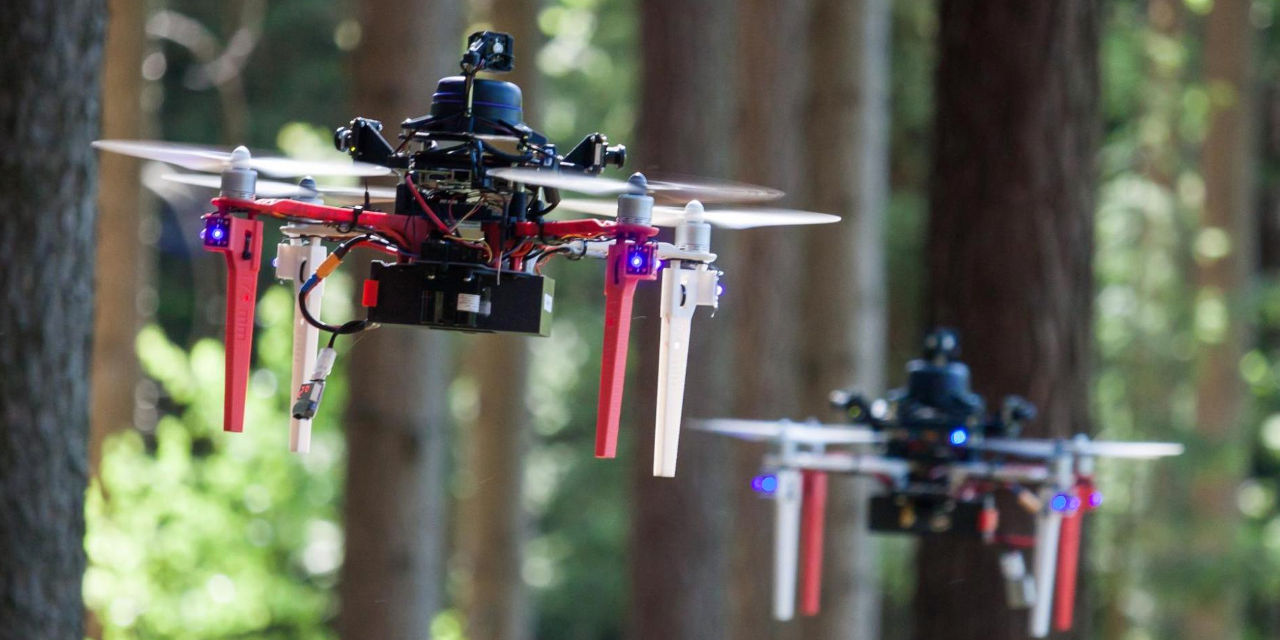
\includegraphics[width=0.345\textwidth]{./fig/photos/uvdar.jpg}};
      \begin{scope}[x={(a.south east)},y={(a.north west)}]
        %%{ grid
        % % useful grid to help you find coordinates for plotting the overlay
        % \draw[black, xstep=.1, ystep=.1] (0,0) grid (1,1);
        % \foreach \i in {0,0.1,0.2,0.3,0.4,0.5,0.6,0.7,0.8,0.9,1} {
        %   \node[align=center] at (\i, -0.05) {\i};
        %   \node[align=center] at (\i, 1.05) {\i};
        %   \node[align=center] at (-0.05, \i) {\i};
        %   \node[align=center] at (1.05, \i) {\i};
        % }
        %%}

        \draw[->, white, thick] (0.40, 0.20) -- (0.18, 0.59);
        \draw[->, white, thick] (0.40, 0.20) -- (0.48, 0.56);
        \draw[->, white, thick] (0.40, 0.20) -- (0.58, 0.24);
        \draw (0.40,0.15) node [text=white] {\small UV blinkers};

        \draw[->, white, thick] (0.80, 0.80) -- (0.80, 0.4);
        \draw[->, white, thick] (0.80, 0.80) -- (0.66, 0.4);
        \draw[->, white, thick] (0.80, 0.80) -- (0.50, 0.77);
        \draw (0.80,0.86) node [text=white] {\small UV cameras};

        % plot some stuff over the image
        \fill[white] (0.001, 0.001) rectangle (0.08,0.13);
        \fill[draw=black, draw opacity=0.5, fill opacity=0] (0,0) rectangle (1, 1);
        \draw (0.04,0.06) node [text=black] {\small (a)};
      \end{scope}
    \end{tikzpicture}}
    \hfill%
    \subfloat {\begin{tikzpicture}
      \node[anchor=south west,inner sep=0] (a) at (0,0) { 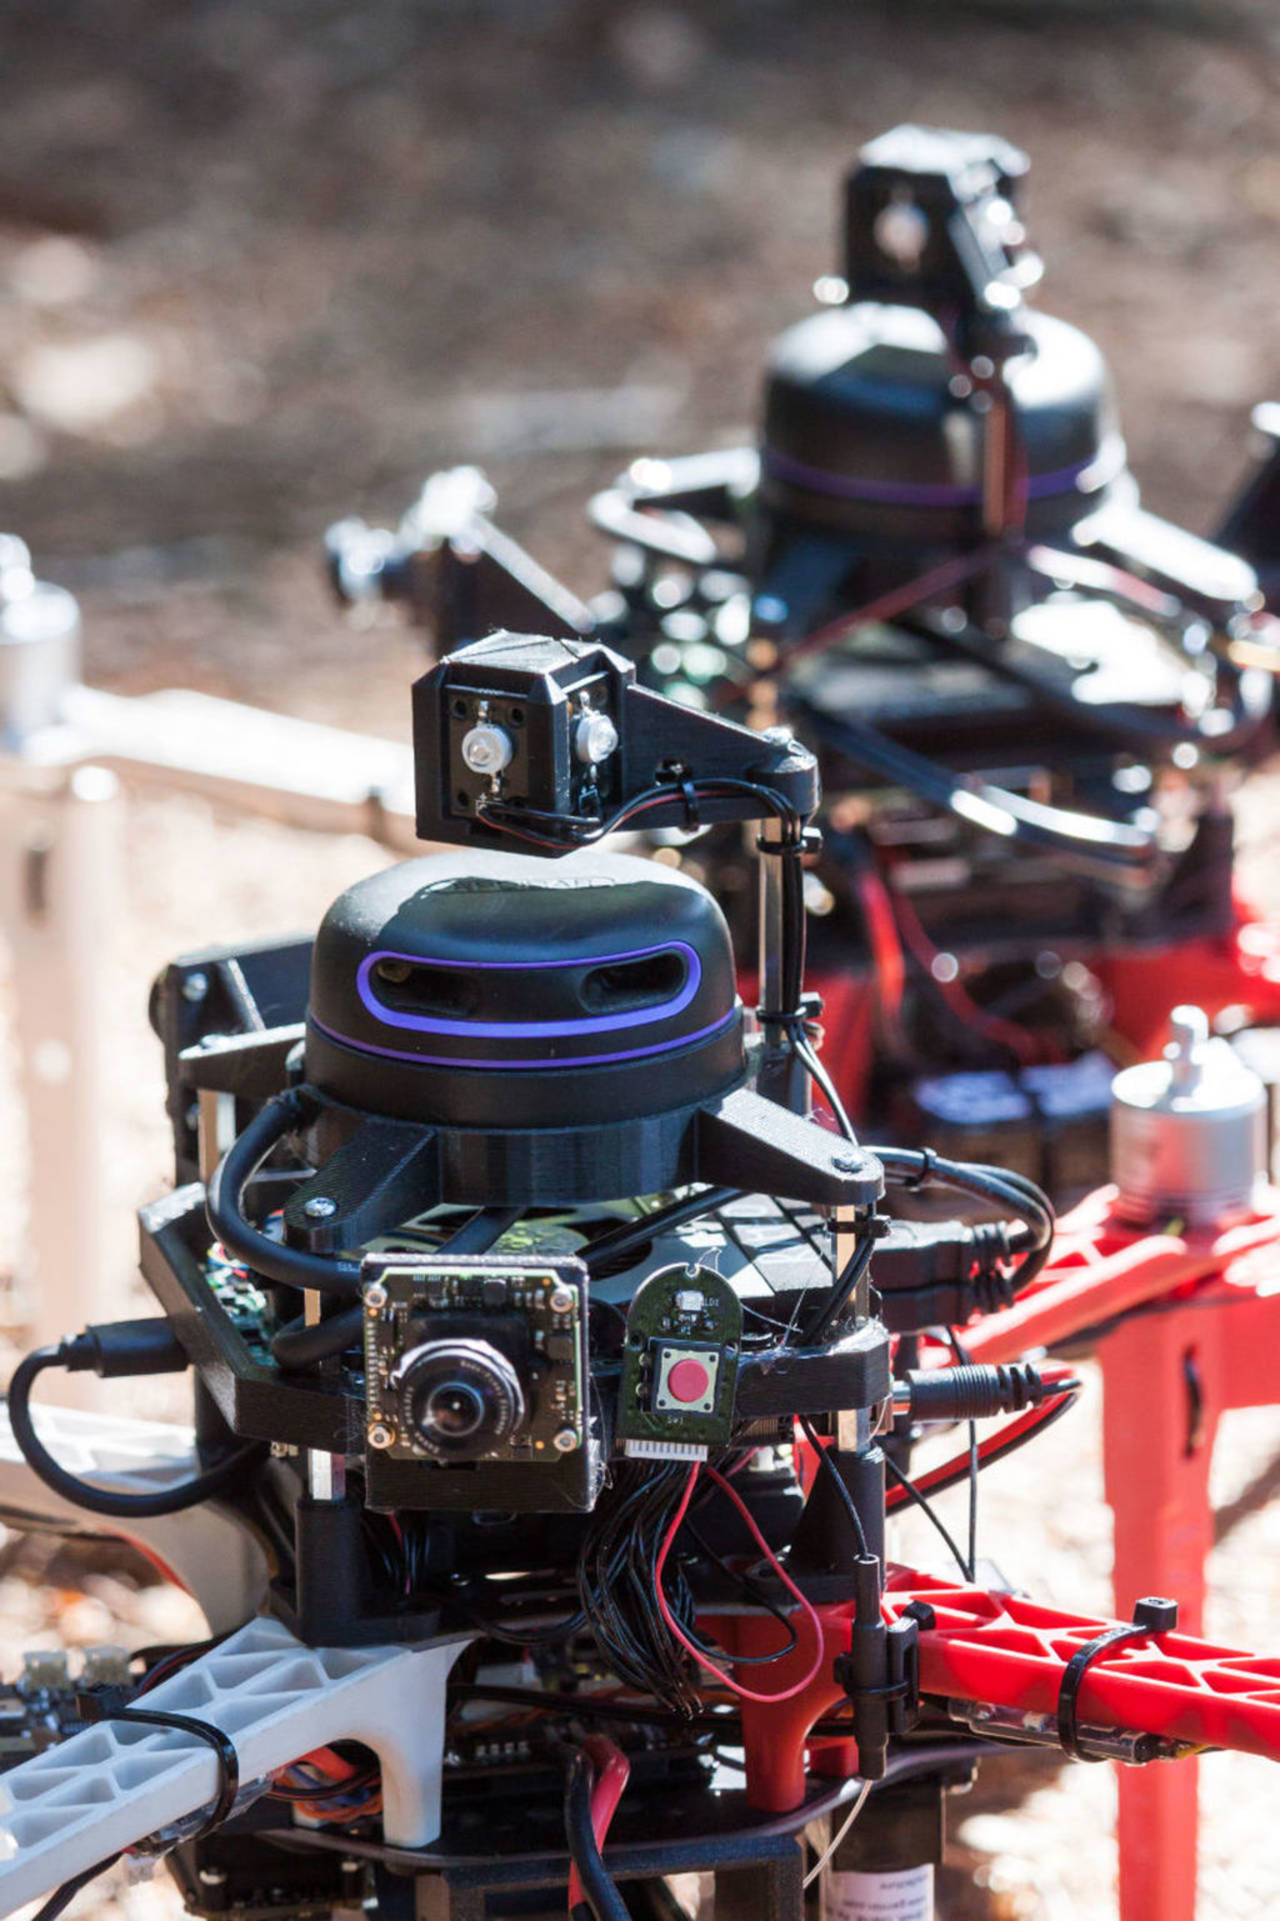
\includegraphics[width=0.115\textwidth]{./fig/photos/uvdar_camera.jpg}};
      \begin{scope}[x={(a.south east)},y={(a.north west)}]
        %%{ grid
        % % useful grid to help you find coordinates for plotting the overlay
        % \draw[black, xstep=.1, ystep=.1] (0,0) grid (1,1);
        % \foreach \i in {0,0.1,0.2,0.3,0.4,0.5,0.6,0.7,0.8,0.9,1} {
        %   \node[align=center] at (\i, -0.05) {\i};
        %   \node[align=center] at (\i, 1.05) {\i};
        %   \node[align=center] at (-0.05, \i) {\i};
        %   \node[align=center] at (1.05, \i) {\i};
        % }
        %%}
        % plot some stuff over the image
        \fill[white] (0.001, 0.001) rectangle (0.20,0.13);
        \fill[draw=black, draw opacity=0.5, fill opacity=0] (0,0) rectangle (1, 1);
        \draw (0.10,0.06) node [text=black] {\small (b)};
      \end{scope}
    \end{tikzpicture}}
    \caption{Mutual localization of \acp{UAV} by the UVDAR system is provided by (a) \ac{UV} blinkers on the \ac{UAV} arms and top. The blinkers are observed by onboard cameras (b) equipped with \ac{UV} band pass filters.}
    \label{fig:uvdar}
  \end{figure}

  \subsection{UAV motion planning}

  Basic research on optimal planning for data collection with \acp{UAV} was studied in \cite{penicka2019data, penicka2017dubins, penicka2017neighborhoods, penicka2017reactive, faigl2017onsolution}.
  The platform provided real-world verification and showed the feasibility of the proposed approaches.
  Coverage optimization for multi-\ac{UAV} cooperative surveillance was tackled in \cite{petrlik2019coverage, faigl2019unsupervised}.
  Complex maneuvers and cooperative load-carrying by multiple \acp{UAV} were reported on in \cite{spurny2019transport, spurny2016complex}.

  \subsection{Automatic control}

  A system for automatic gain tuning for the \emph{SE(3) controller} (see \refsec{sec:se3_state_feedback}) was published in \cite{giernacky2019realtime}.
  A novel optimal control design approach for automatic fire extinguishing is showcased in \cite{saikin2020wildfire}.
  The properties of the SE(3) geometric feedback proved crucial for verifying the feasibility of the almost-free-fall trajectories designed to dispatch water during extreme maneuvers (see \reffig{fig:control}).

  \begin{figure}
    \centering
    \subfloat {\begin{tikzpicture}
      \node[anchor=south west,inner sep=0] (a) at (0,0) { 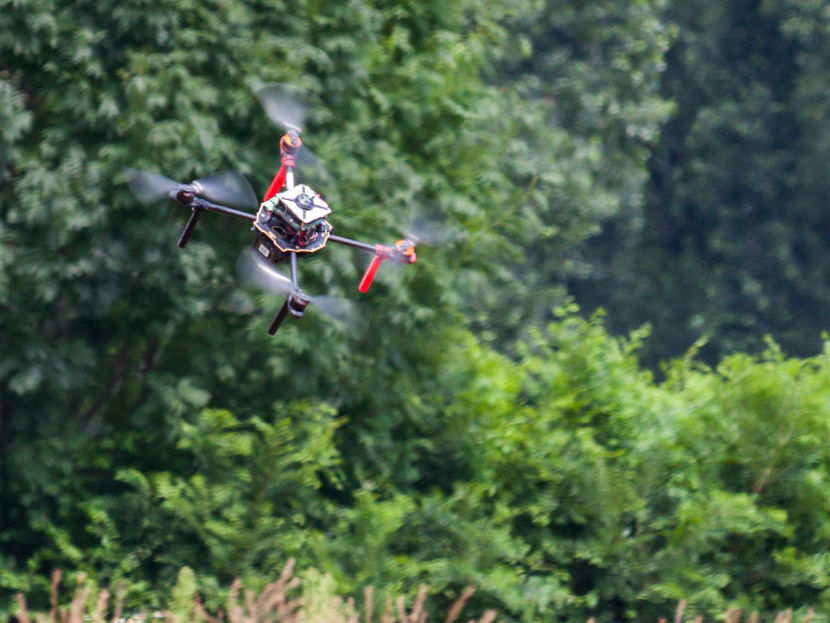
\includegraphics[width=0.235\textwidth]{./fig/photos/control_2_1-5.jpg}};
      \begin{scope}[x={(a.south east)},y={(a.north west)}]
        %%{ grid
        % % useful grid to help you find coordinates for plotting the overlay
        % \draw[black, xstep=.1, ystep=.1] (0,0) grid (1,1);
        % \foreach \i in {0,0.1,0.2,0.3,0.4,0.5,0.6,0.7,0.8,0.9,1} {
        %   \node[align=center] at (\i, -0.05) {\i};
        %   \node[align=center] at (\i, 1.05) {\i};
        %   \node[align=center] at (-0.05, \i) {\i};
        %   \node[align=center] at (1.05, \i) {\i};
        % }
        %%}
        % plot some stuff over the image
        \fill[white] (0.001, 0.001) rectangle (0.12,0.13);
        \fill[draw=black, draw opacity=0.5, fill opacity=0] (0,0) rectangle (1, 1);
        \draw (0.06,0.06) node [text=black] {\small (a)};
      \end{scope}
    \end{tikzpicture}}
    \hfill%
    \subfloat {\begin{tikzpicture}
      \node[anchor=south west,inner sep=0] (a) at (0,0) { 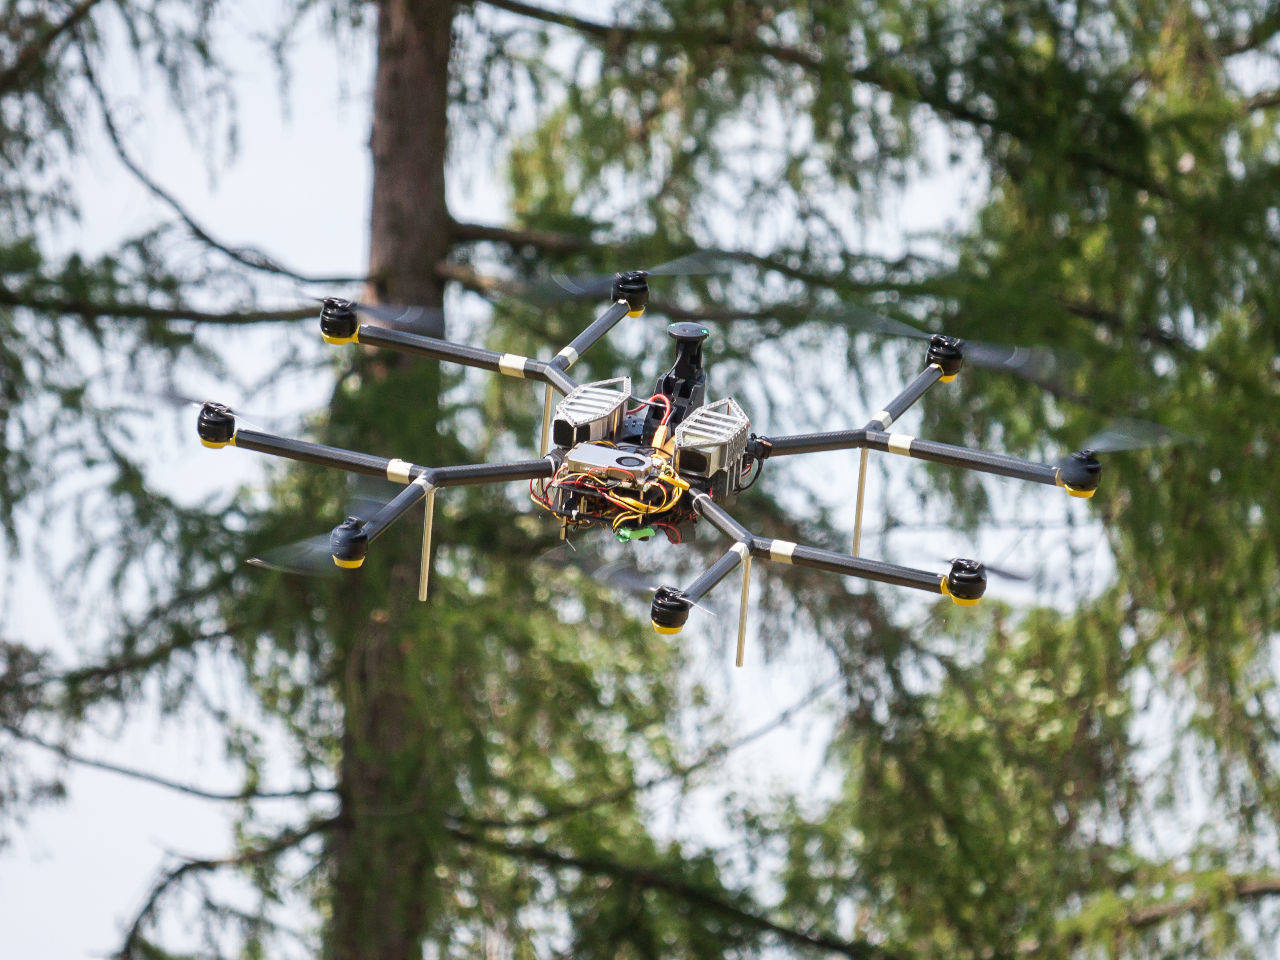
\includegraphics[width=0.235\textwidth]{./fig/photos/eagle_2_1-5.jpg}};
      \begin{scope}[x={(a.south east)},y={(a.north west)}]
        %%{ grid
        % % useful grid to help you find coordinates for plotting the overlay
        % \draw[black, xstep=.1, ystep=.1] (0,0) grid (1,1);
        % \foreach \i in {0,0.1,0.2,0.3,0.4,0.5,0.6,0.7,0.8,0.9,1} {
        %   \node[align=center] at (\i, -0.05) {\i};
        %   \node[align=center] at (\i, 1.05) {\i};
        %   \node[align=center] at (-0.05, \i) {\i};
        %   \node[align=center] at (1.05, \i) {\i};
        % }
        %%}
        % plot some stuff over the image
        \fill[white] (0.001, 0.001) rectangle (0.12,0.13);
        \fill[draw=black, draw opacity=0.5, fill opacity=0] (0,0) rectangle (1, 1);
        \draw (0.06,0.06) node [text=black] {\small (b)};
      \end{scope}
    \end{tikzpicture}}
    \caption{Novel control approaches can be tested on a real hardware. Off-the-shelf platforms such as (a) Tarot 650, and also (b) custom-built airframes, can be equipped with the proposed system.}
    \label{fig:control}
  \end{figure}

  \subsection{Data gathering}

  The system is being used actively in a project working on indoor aerial inspection of historical buildings and monuments \cite{petracek2020dronument, saska2017documentation, kratky2020autonomous}.
  Within this scenario, a \ac{UAV} is equipped with a 3D \ac{LiDAR} sensor and is automatically guided through an indoor environment, where it captures detailed imagery of hard-to-reach points of interest (see \reffig{fig:dronument}).
  In another project\footnote{\url{http://mrs.felk.cvut.cz/radron}}, ionizing radiation mapping and localization is studied in \cite{baca2018rospix, baca2019timepix, stibinger2020localization}.
  Similarly, transmission radio sources were automatically localized in \cite{vrba2019realtime}.

  \begin{figure}
    \centering
    \subfloat {\begin{tikzpicture}
      \node[anchor=south west,inner sep=0] (a) at (0,0) { 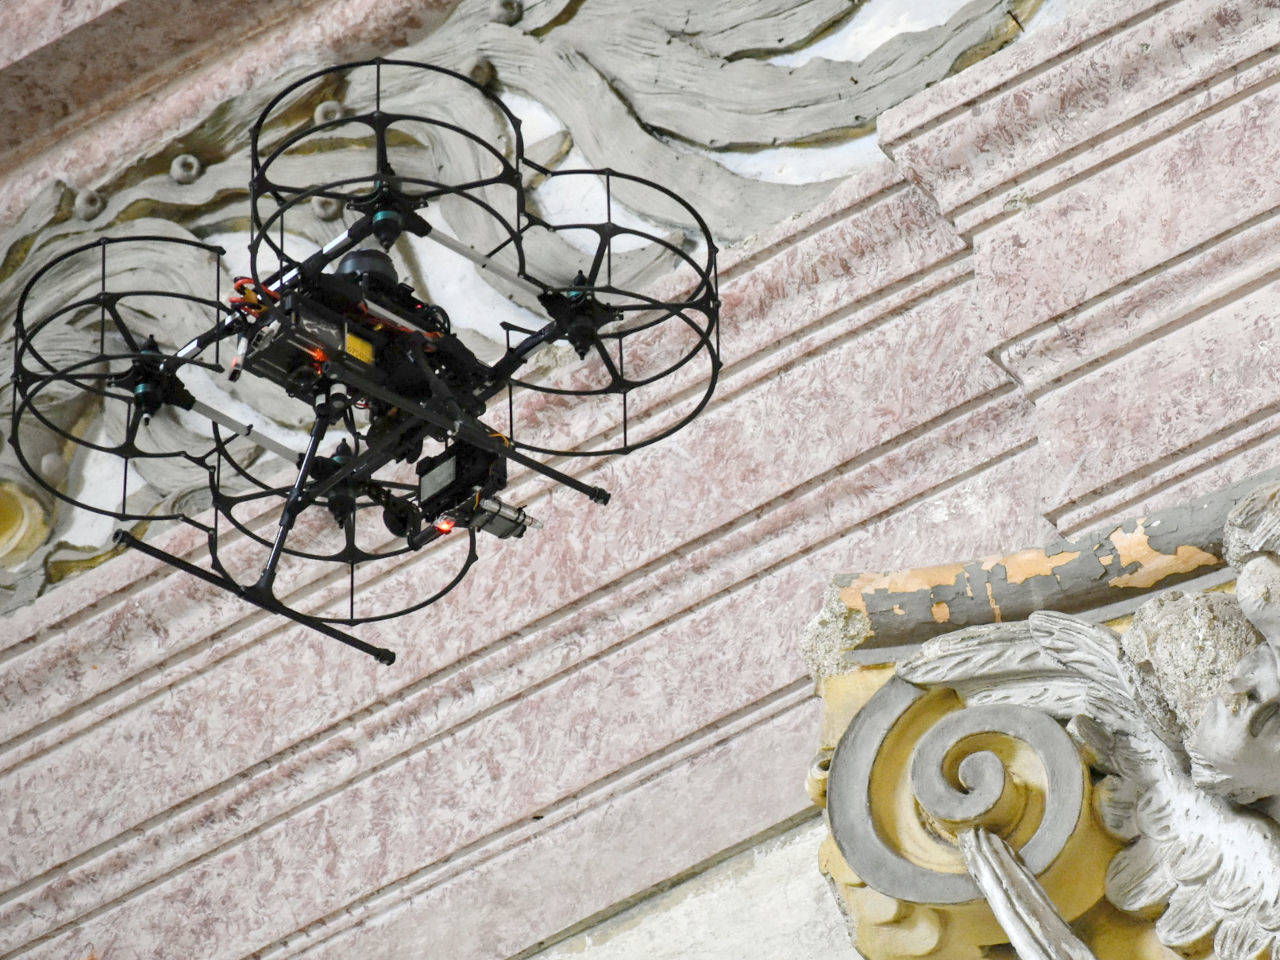
\includegraphics[width=0.235\textwidth]{./fig/photos/dronument_2_2_1-5.jpg}};
      \begin{scope}[x={(a.south east)},y={(a.north west)}]
        %%{ grid
        % % useful grid to help you find coordinates for plotting the overlay
        % \draw[black, xstep=.1, ystep=.1] (0,0) grid (1,1);
        % \foreach \i in {0,0.1,0.2,0.3,0.4,0.5,0.6,0.7,0.8,0.9,1} {
        %   \node[align=center] at (\i, -0.05) {\i};
        %   \node[align=center] at (\i, 1.05) {\i};
        %   \node[align=center] at (-0.05, \i) {\i};
        %   \node[align=center] at (1.05, \i) {\i};
        % }
        %%}
        % plot some stuff over the image
        \fill[white] (0.001, 0.001) rectangle (0.12,0.13);
        \fill[draw=black, draw opacity=0.5, fill opacity=0] (0,0) rectangle (1, 1);
        \draw (0.06,0.06) node [text=black] {\small (a)};
      \end{scope}
    \end{tikzpicture}}
    \hfill%
    \subfloat {\begin{tikzpicture}
      \node[anchor=south west,inner sep=0] (a) at (0,0) { 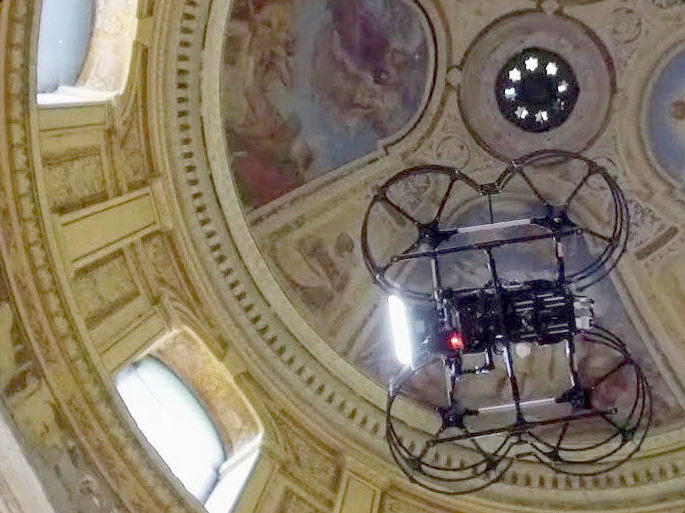
\includegraphics[width=0.235\textwidth]{./fig/photos/dronument_2_1-5.jpg}};
      \begin{scope}[x={(a.south east)},y={(a.north west)}]
        %%{ grid
        % % useful grid to help you find coordinates for plotting the overlay
        % \draw[black, xstep=.1, ystep=.1] (0,0) grid (1,1);
        % \foreach \i in {0,0.1,0.2,0.3,0.4,0.5,0.6,0.7,0.8,0.9,1} {
        %   \node[align=center] at (\i, -0.05) {\i};
        %   \node[align=center] at (\i, 1.05) {\i};
        %   \node[align=center] at (-0.05, \i) {\i};
        %   \node[align=center] at (1.05, \i) {\i};
        % }
        %%}
        % plot some stuff over the image
        \fill[white] (0.001, 0.001) rectangle (0.12,0.13);
        \fill[draw=black, draw opacity=0.5, fill opacity=0] (0,0) rectangle (1, 1);
        \draw (0.06,0.06) node [text=black] {\small (b)};
      \end{scope}
    \end{tikzpicture}}
    \caption{An inspection of an indoor historical building is conducted (a) to monitor the state of frescoes, and (b) to assess the state of wall paintings.}
    \label{fig:dronument}
  \end{figure}

  \subsection{UAV swarms and formations}
  \label{sec:uav_swarms_and_formations}

  Basic research in the area of \ac{UAV} swarming and formation flying was studied in \cite{saska2020formation, saska2016formations, saska2019large}.
  UAV swarm control is a relatively new field of research, and its applications are yet to be explored.
  One of many possibilities being explored by the authors is the use of \acp{UAV} for inspecting hard-to-access locations such as power line towers without putting personnel at risk\footnote{\url{https://aerial-core.eu}}.
  % The need for a swarm of \acp{UAV} is essential in this type of application.
  This type of application requires the swarm coordination to be flexible, and to move, while minimizing the observed object estimation error.
  % A crucial piece of information required for coordination of multi-robot systems working in the same workspace is a precise knowledge of mutual states of teammates.
  Flocking capabilities are being explored within the framework of ongoing projects with real-world experiments in a field, and also within a forest environment (see \reffig{fig:swarms}).
  Interactions between \acp{UAV} are studied in order to overcome challenging situations such as GNSS-denied environment navigation.

  \begin{figure}
    \centering
    \subfloat {\begin{tikzpicture}
      \node[anchor=south west,inner sep=0] (a) at (0,0) { 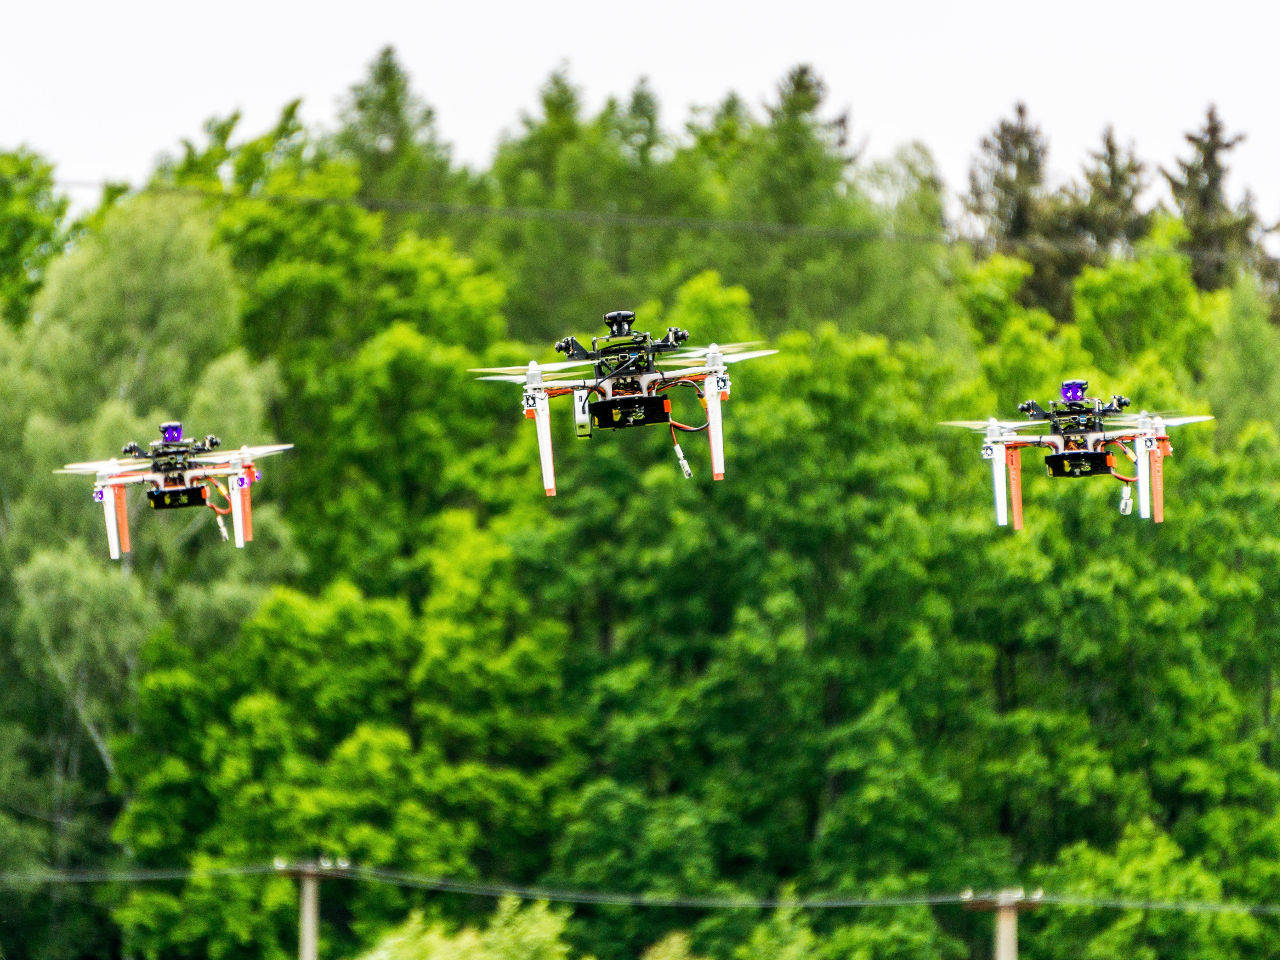
\includegraphics[width=0.235\textwidth]{./fig/photos/swarm_2_1-5.jpg}};
      \begin{scope}[x={(a.south east)},y={(a.north west)}]
        %%{ grid
        % % useful grid to help you find coordinates for plotting the overlay
        % \draw[black, xstep=.1, ystep=.1] (0,0) grid (1,1);
        % \foreach \i in {0,0.1,0.2,0.3,0.4,0.5,0.6,0.7,0.8,0.9,1} {
        %   \node[align=center] at (\i, -0.05) {\i};
        %   \node[align=center] at (\i, 1.05) {\i};
        %   \node[align=center] at (-0.05, \i) {\i};
        %   \node[align=center] at (1.05, \i) {\i};
        % }
        %%}
        \fill[white] (0.001, 0.001) rectangle (0.12,0.13);
        % plot some stuff over the image
        \fill[draw=black, draw opacity=0.5, fill opacity=0] (0,0) rectangle (1, 1);
        \draw (0.06,0.06) node [text=black] {\small (a)};
      \end{scope}
    \end{tikzpicture}}
    \hfill
    \subfloat {\begin{tikzpicture}
      \node[anchor=south west,inner sep=0] (a) at (0,0) { 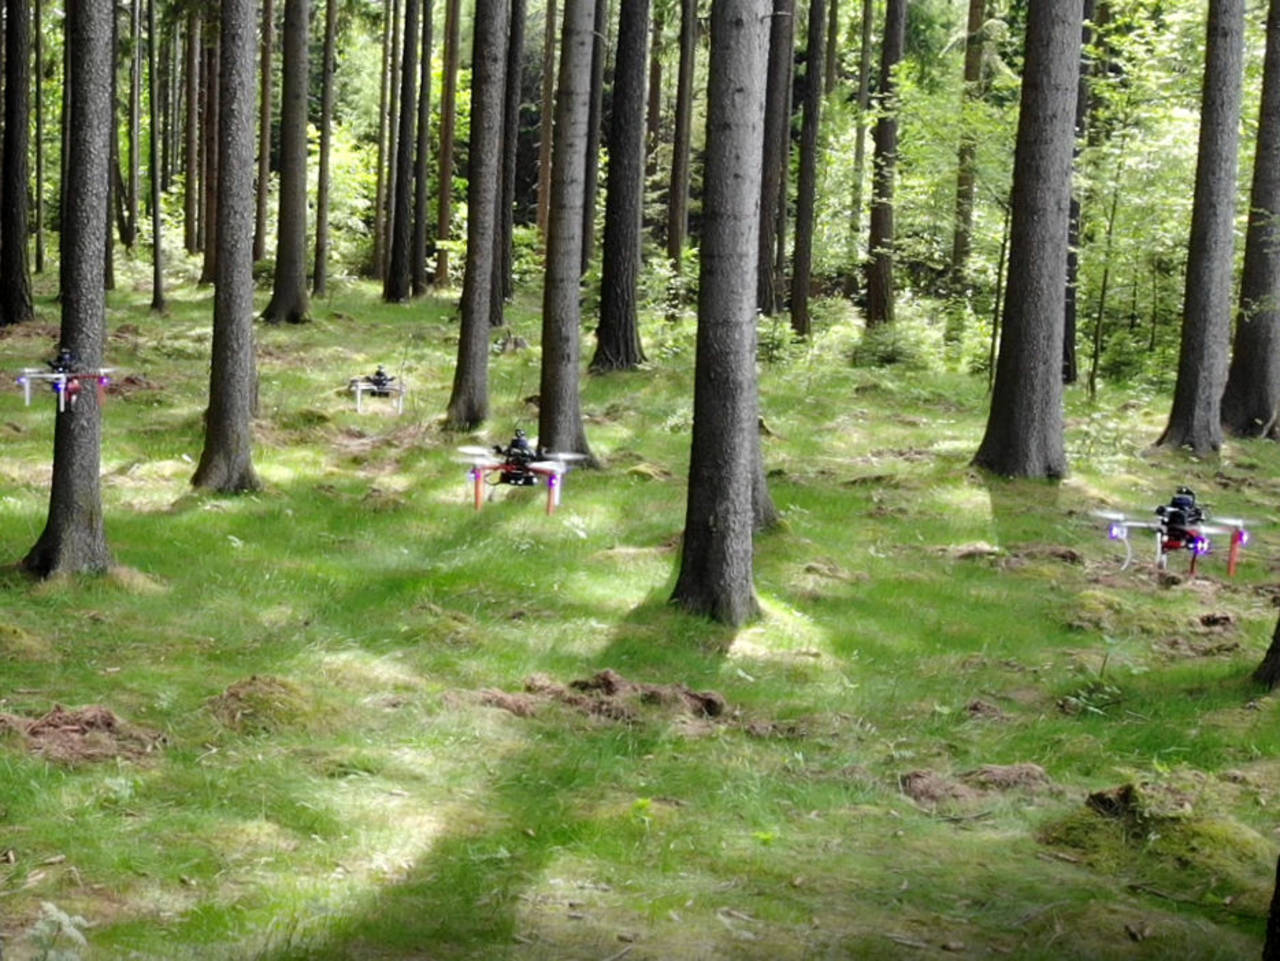
\includegraphics[width=0.235\textwidth]{./fig/photos/swarm_forest_2_1-5.jpg}};
      \begin{scope}[x={(a.south east)},y={(a.north west)}]
        %%{ grid
        % useful grid to help you find coordinates for plotting the overlay
        % \draw[black, xstep=.1, ystep=.1] (0,0) grid (1,1);
        % \foreach \i in {0,0.1,0.2,0.3,0.4,0.5,0.6,0.7,0.8,0.9,1} {
        %   \node[align=center] at (\i, -0.05) {\i};
        %   \node[align=center] at (\i, 1.05) {\i};
        %   \node[align=center] at (-0.05, \i) {\i};
        %   \node[align=center] at (1.05, \i) {\i};
        % }
        %%}

        \draw[->, white, thick] (0.45, 0.20) -- (0.07, 0.57);
        \draw[->, white, thick] (0.45, 0.20) -- (0.30, 0.55);
        \draw[->, white, thick] (0.45, 0.20) -- (0.40, 0.45);
        \draw[->, white, thick] (0.45, 0.20) -- (0.85, 0.40);
        \draw (0.45,0.15) node [text=white] {\small UAVs};

        \fill[white] (0.001, 0.001) rectangle (0.12,0.13);
        % plot some stuff over the image
        \fill[draw=black, draw opacity=0.5, fill opacity=0] (0,0) rectangle (1, 1);
        \draw (0.06,0.06) node [text=black] {\small (b)};
      \end{scope}
    \end{tikzpicture}}
    \caption{Swarms of multirotor \acp{UAV} testing novel flocking algorithms while localized (a) by a \ac{GNSS} system, and (b) by onboard sensors only within a forest environment.}
    \label{fig:swarms}
  \end{figure}

  % Most cited approaches, although achieving great results, lack reliability in terms of independence to changing environmental conditions in the real-world, which is not acceptable in such the proposed safety-critical work. This means that a fully distributed control approach is needed. To achieve that, we plan to apply our achievements in the endeavor to design a robust system usable in various environments, both relying on vision-based precise mutual object detection in UAV proximity \cite{krajnik14jint} as well as using robust active UV patterns to solve this problem \cite{Walter2018}.

  \subsection{MBZIRC 2017 competition}

  The \ac{MBZIRC} 2017\footnote{MBZIRC 2017, \url{http://mbzirc.com/challenge/2017}} aimed at pushing the frontiers of field robotics.
  Two tasks out of the three challenges within the competition were focused solely on aerial manipulation and UAV control.
  The competition imposed real-world constraints in its tasks that forced the participating teams to show the current state of the art in robotics and to perform the tasks within a short time window and within specified time slots.
  The first task --- autonomous gathering of colored ferrous objects by a group of \acp{UAV} --- was successfully tackled by the CTU-UPENN-UoL\footnote{Collaboration of Czech Technical University in Prague, University of Pennsylvania, and the University of Lincoln.} team, using the proposed system \cite{spurny2019cooperative, faigl2019unsupervised, loianno2018localization} (see \reffig{fig:mbzirc_2017}).
  We won 1$^{\mathrm{st}}$ place among the best teams from all over the world.
  The second task of autonomous landing on a moving car was also tackled by the proposed system.
  We achieved the fastest autonomous landing among all the teams, and we took the 2$^{\text{nd}}$ place overall in the competition \cite{baca2019autonomous, stepan2019vision}.

  \begin{figure}
    \centering
    \subfloat {\begin{tikzpicture}
      \node[anchor=south west,inner sep=0] (a) at (0,0) { 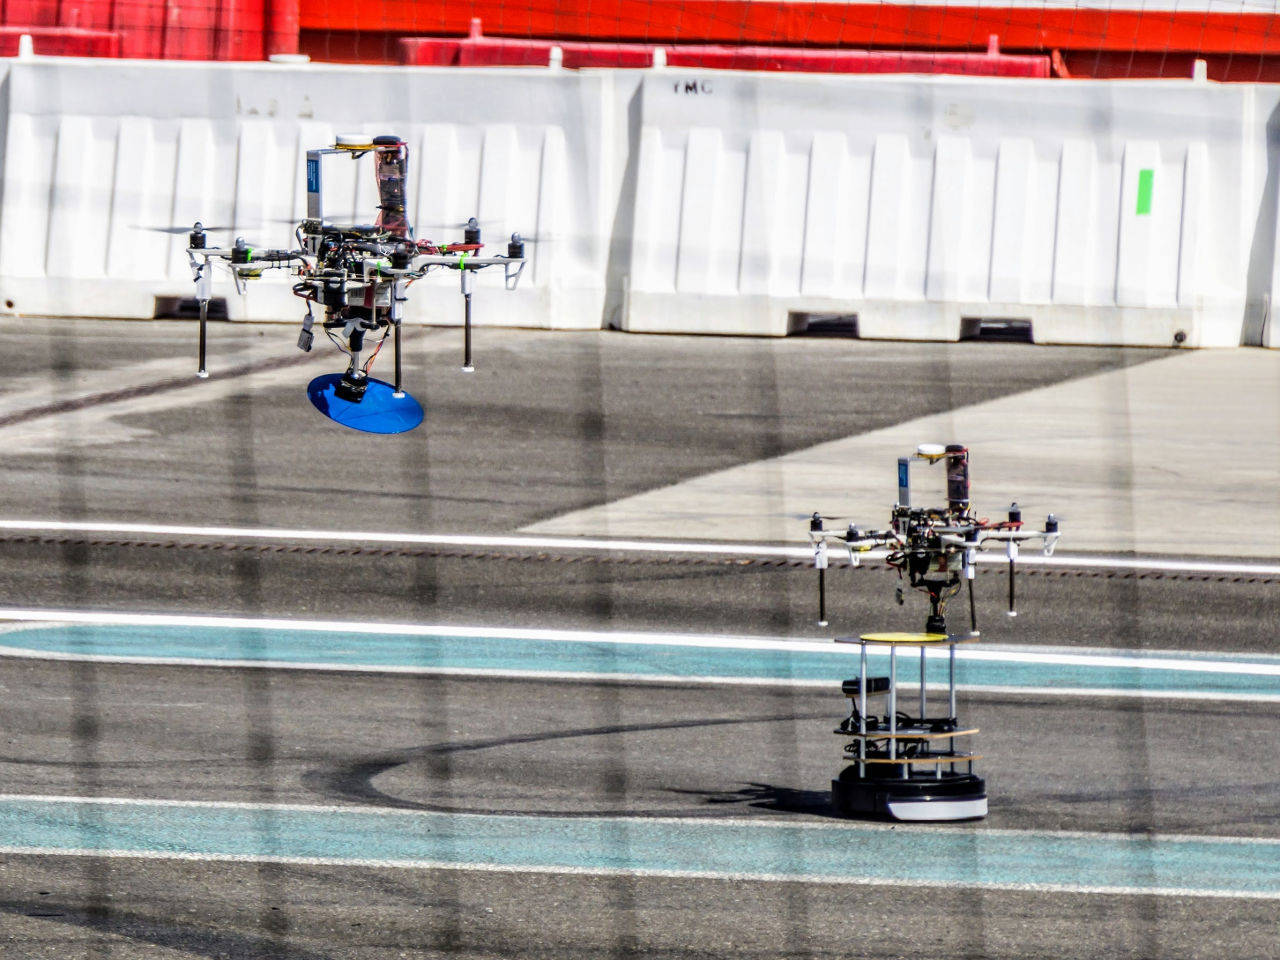
\includegraphics[width=0.235\textwidth]{./fig/photos/grasping_2017_2_1-5.jpg}};
      \begin{scope}[x={(a.south east)},y={(a.north west)}]
        %%{ grid
        % % useful grid to help you find coordinates for plotting the overlay
        % \draw[black, xstep=.1, ystep=.1] (0,0) grid (1,1);
        % \foreach \i in {0,0.1,0.2,0.3,0.4,0.5,0.6,0.7,0.8,0.9,1} {
        %   \node[align=center] at (\i, -0.05) {\i};
        %   \node[align=center] at (\i, 1.05) {\i};
        %   \node[align=center] at (-0.05, \i) {\i};
        %   \node[align=center] at (1.05, \i) {\i};
        % }
        %%}
        % plot some stuff over the image
        \fill[white] (0.001, 0.001) rectangle (0.12,0.13);
        \fill[draw=black, draw opacity=0.5, fill opacity=0] (0,0) rectangle (1, 1);
        \draw (0.06,0.06) node [text=black] {\small (a)};
      \end{scope}
    \end{tikzpicture}}
    \hfill%
    \subfloat {\begin{tikzpicture}
      \node[anchor=south west,inner sep=0] (a) at (0,0) { 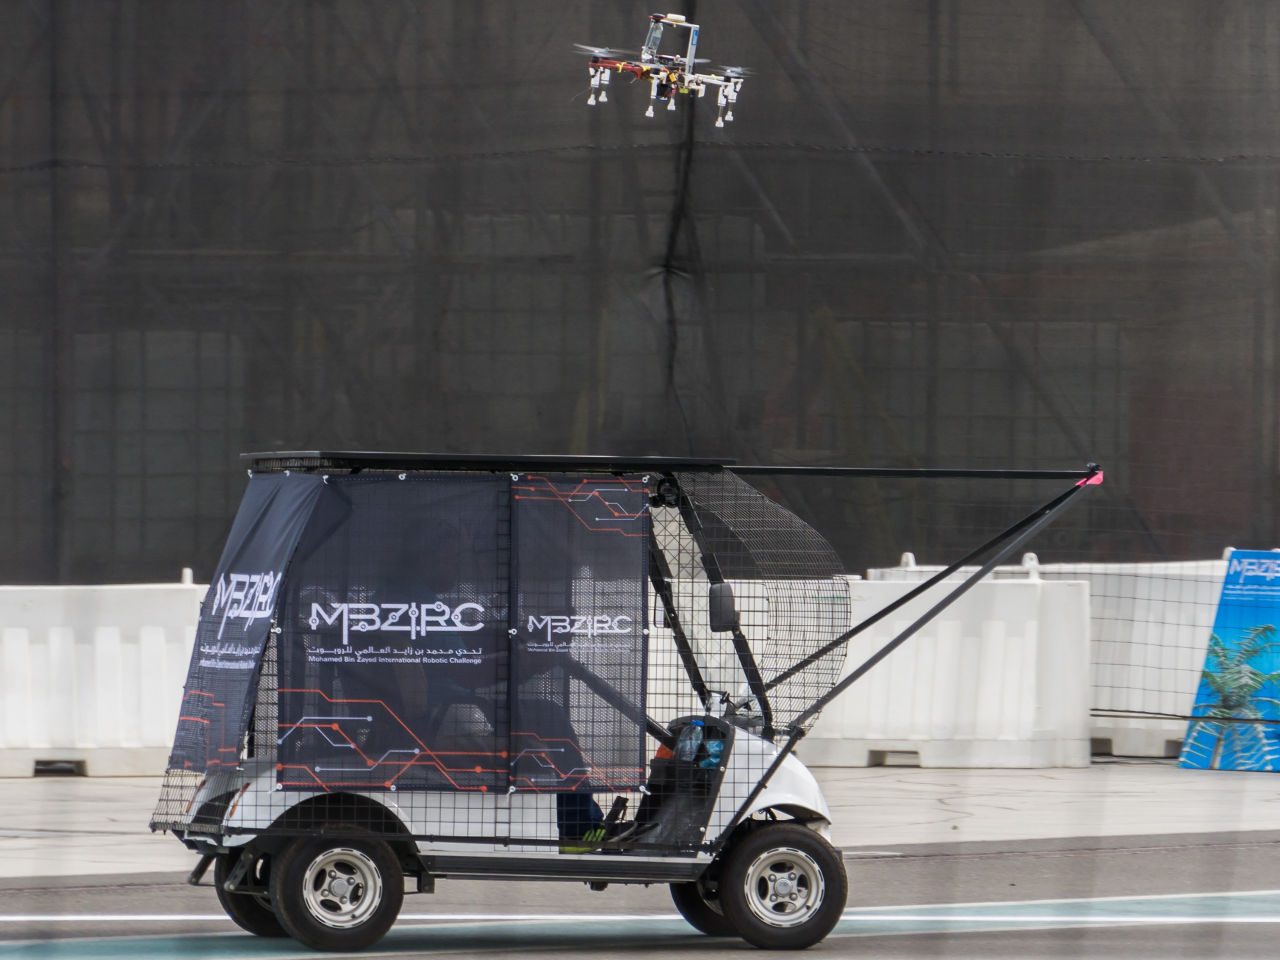
\includegraphics[width=0.235\textwidth]{./fig/photos/landing_2017_2_1-5.jpg}};
      \begin{scope}[x={(a.south east)},y={(a.north west)}]
        %%{ grid
        % % useful grid to help you find coordinates for plotting the overlay
        % \draw[black, xstep=.1, ystep=.1] (0,0) grid (1,1);
        % \foreach \i in {0,0.1,0.2,0.3,0.4,0.5,0.6,0.7,0.8,0.9,1} {
        %   \node[align=center] at (\i, -0.05) {\i};
        %   \node[align=center] at (\i, 1.05) {\i};
        %   \node[align=center] at (-0.05, \i) {\i};
        %   \node[align=center] at (1.05, \i) {\i};
        % }
        %%}
        % plot some stuff over the image
        \fill[white] (0.001, 0.001) rectangle (0.12,0.13);
        \fill[draw=black, draw opacity=0.5, fill opacity=0] (0,0) rectangle (1, 1);
        \draw (0.06,0.06) node [text=black] {\small (b)};
      \end{scope}
    \end{tikzpicture}}
    \caption{The CTU-UPENN-UoL team during the MBZIRC 2017 competition. The photos show (a) two \acp{UAV} while delivering ferrous objects, and (b) a UAV during autonomous landing on a moving car.}
    \label{fig:mbzirc_2017}
  \end{figure}

  \subsection{The DARPA Subterranean (SubT) challenge}

  The \ac{DARPA}, an agency of the United States Department of Defense, organizes series of challenges focused on automatic search \& rescue in an underground environment --- the \ac{DARPA} Subterranean challenge.
  In the \ac{DARPA} Tunnel Circuit, the first round of the challenge, we deployed autonomous \acp{UAV} and semi-autonomous ground robots to explore underground mine shafts \cite{petrlik2020robust, roucek2019darpa}.
  Our team deployed autonomous \acp{UAV} with the proposed system (see \reffig{fig:darpa}), which navigated the underground tunnels and returned safely to the entrance while autonomously localizing objects of interest.
  We won the 1$^{\mathrm{st}}$ prize among the self-funded teams and the 3$^{\mathrm{rd}}$ prize overall.
  To the best of our knowledge, our \acp{UAV} managed to explore a greater distance into the tunnels than any of the other teams.
  \begin{figure}
    \centering
    \subfloat {\begin{tikzpicture}
      \node[anchor=south west,inner sep=0] (a) at (0,0) { 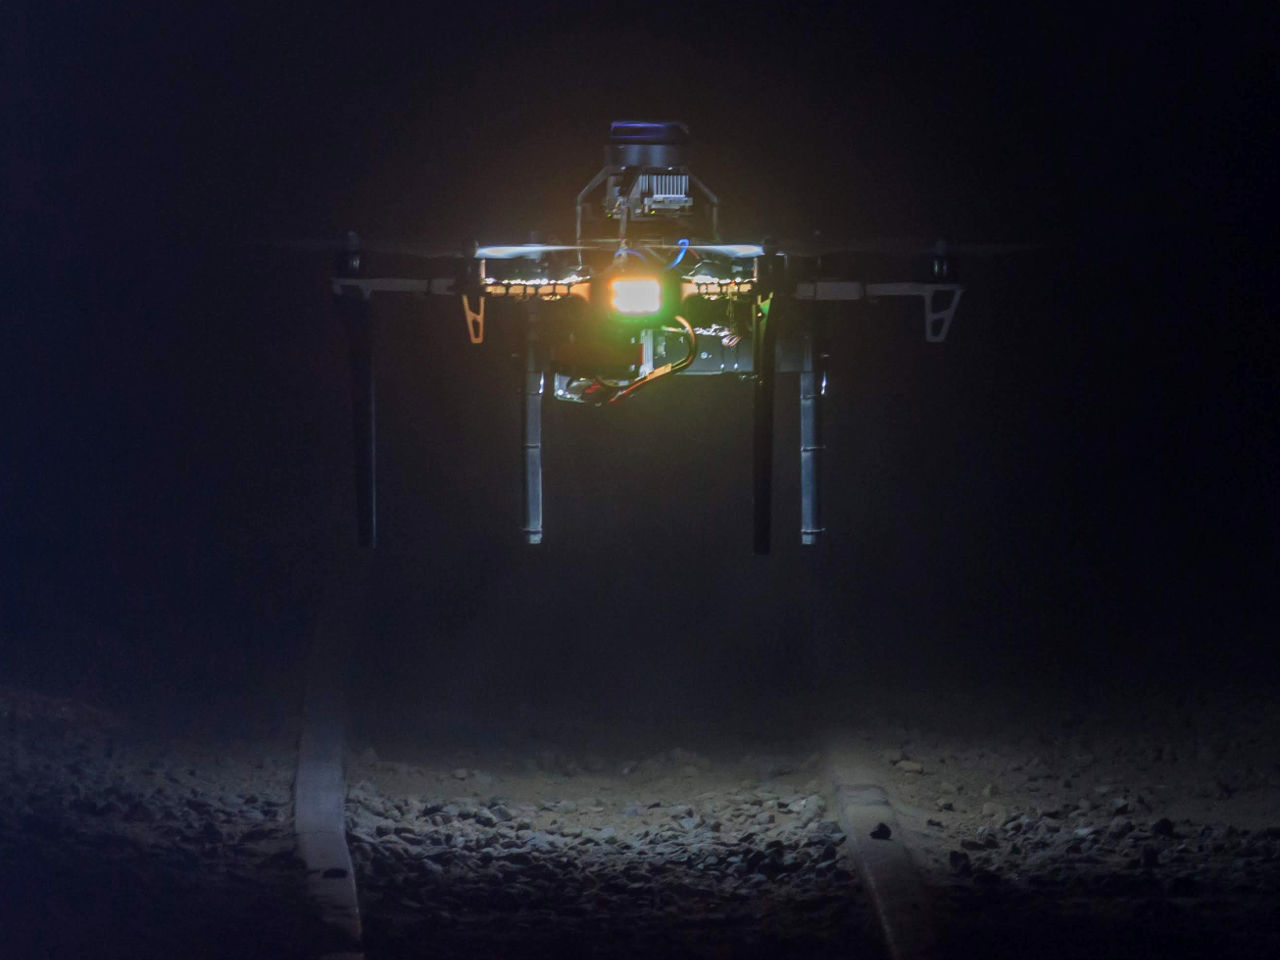
\includegraphics[width=0.235\textwidth]{./fig/photos/darpa_stix_2_1-5.jpg}};
      \begin{scope}[x={(a.south east)},y={(a.north west)}]
        %%{ grid
        % % useful grid to help you find coordinates for plotting the overlay
        % \draw[black, xstep=.1, ystep=.1] (0,0) grid (1,1);
        % \foreach \i in {0,0.1,0.2,0.3,0.4,0.5,0.6,0.7,0.8,0.9,1} {
        %   \node[align=center] at (\i, -0.05) {\i};
        %   \node[align=center] at (\i, 1.05) {\i};
        %   \node[align=center] at (-0.05, \i) {\i};
        %   \node[align=center] at (1.05, \i) {\i};
        % }
        %%}
        % plot some stuff over the image
        \fill[white] (0.001, 0.001) rectangle (0.12,0.13);
        \fill[draw=black, draw opacity=0.5, fill opacity=0] (0,0) rectangle (1, 1);
        \draw (0.06,0.06) node [text=black] {\small (a)};
      \end{scope}
    \end{tikzpicture}}
    \hfill%
    \subfloat {\begin{tikzpicture}
      \node[anchor=south west,inner sep=0] (a) at (0,0) { 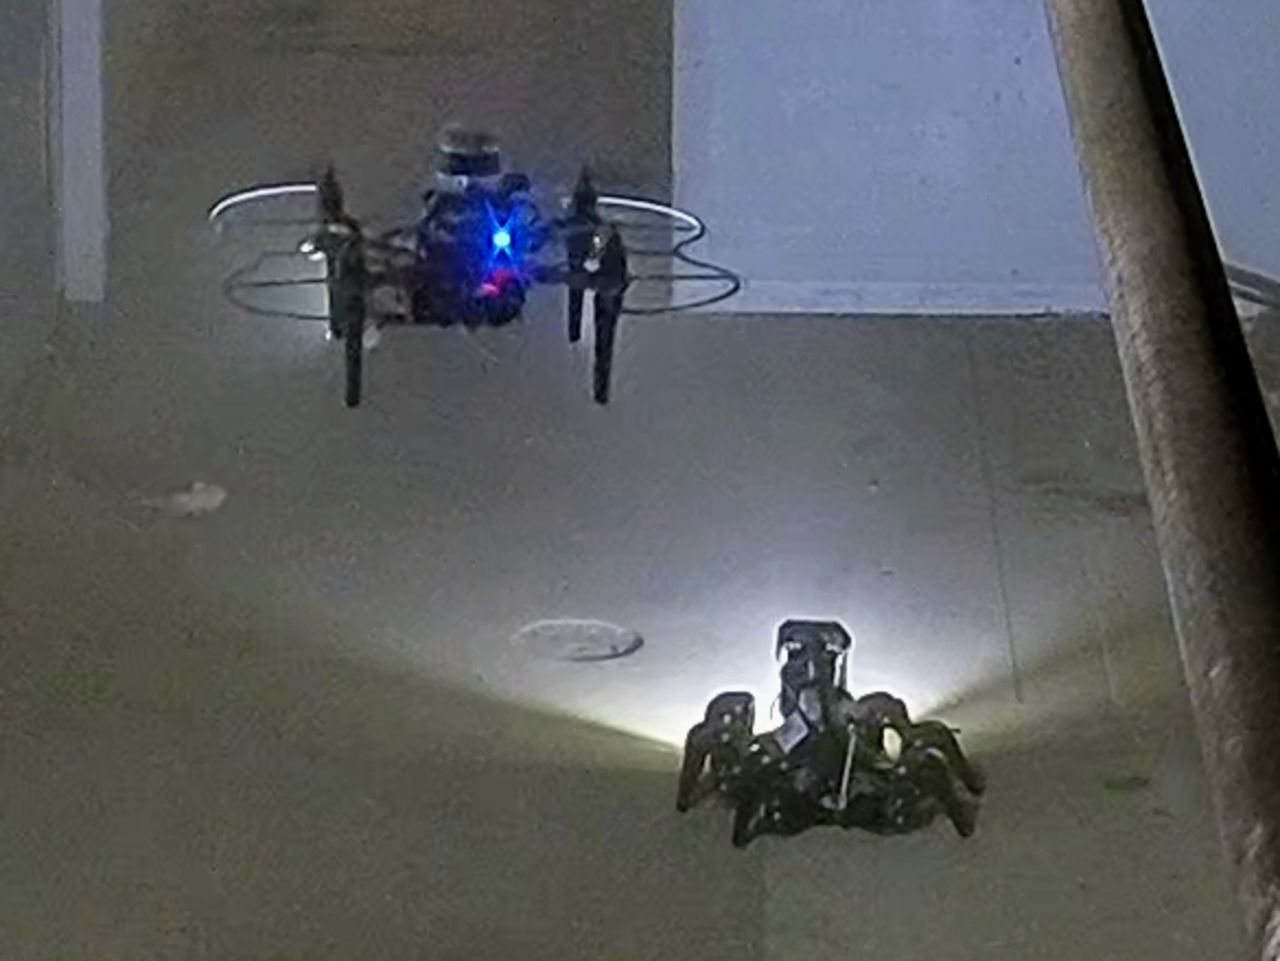
\includegraphics[width=0.235\textwidth]{./fig/photos/darpa_drone_beta_2_1-5.jpg}};
      \begin{scope}[x={(a.south east)},y={(a.north west)}]
        %%{ grid
        % % useful grid to help you find coordinates for plotting the overlay
        % \draw[black, xstep=.1, ystep=.1] (0,0) grid (1,1);
        % \foreach \i in {0,0.1,0.2,0.3,0.4,0.5,0.6,0.7,0.8,0.9,1} {
        %   \node[align=center] at (\i, -0.05) {\i};
        %   \node[align=center] at (\i, 1.05) {\i};
        %   \node[align=center] at (-0.05, \i) {\i};
        %   \node[align=center] at (1.05, \i) {\i};
        % }
        %%}
        % plot some stuff over the image
        \fill[white] (0.001, 0.001) rectangle (0.12,0.13);
        \fill[draw=black, draw opacity=0.5, fill opacity=0] (0,0) rectangle (1, 1);
        \draw (0.06,0.06) node [text=black] {\small (b)};
      \end{scope}
    \end{tikzpicture}}
    \caption{Unmanned Aerial Vehicles during the \ac{DARPA} SubT challenge. The photos depict (a) a UAV exploring an underground mine, and (b) mapping an unfinished nuclear power plant.}
    \label{fig:darpa}
  \end{figure}

  In the \ac{DARPA} Urban Circuit, the second round of the challenge, we deployed autonomous \acp{UAV} and semi-autonomous ground robots to explore the infrastructure of an unfinished nuclear power plant.
  Our \acp{UAV} managed to explore \SI{2867}{\meter\cubed} of one floor of the reactor building while automatically navigating up to \SI{100}{\meter} in just \SI{200}{\second} in a completely unknown environment.
  We again took 1$^{\text{st}}$ place among the self-funded teams, and 3$^{\text{rd}}$ place overall.
  Scientific publications on tasks within the Urban Circuit are under preparation.

  \subsection{MBZIRC 2020 competition}

  The second round of the \ac{MBZIRC} competition was organized in 2020.
  It pushed the current state of the art in aerial robotics to its limits, with tasks such as organizing a group of \acp{UAV} and a \ac{UGV} to build a brick wall autonomously, autonomous indoor and outdoor firefighting with \acp{UAV}, and autonomously catching a ball carried by a \ac{UAV}, performed simultaneously with balloon popping by a group of \acp{UAV} (see \reffig{fig:mbzirc_2020}).
  All of the tasks were solved using the proposed UAV system, and our participation in the competition helped to consolidate many of the platform's functionalities.
  The CTU-UPENN-NYU\footnote{Collaboration between the Czech Technical University in Prague, the University of Pennsylvania, and the New York University.} team achieved the highest score of all the teams for building the brick wall autonomously.
  We also took $2^{\text{nd}}$ in the autonomous balloon popping and ball-catching task.
  We won the gold medal in the \emph{grand challenge} in which all the tasks were tested simultaneously.
  Scientific publications reporting on \ac{MBZIRC} 2020 are under preparation.

  \begin{figure}
    \centering
    \subfloat {\begin{tikzpicture}
      \node[anchor=south west,inner sep=0] (a) at (0,0) { 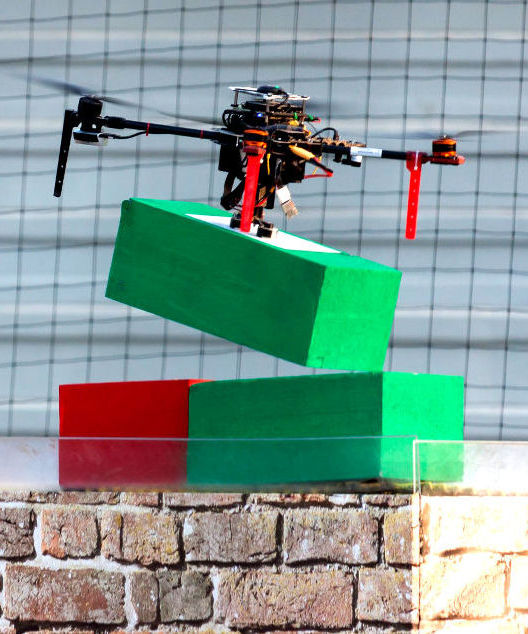
\includegraphics[width=0.155\textwidth]{./fig/photos/brick_placing_1-25_1-5.jpg}};
      \begin{scope}[x={(a.south east)},y={(a.north west)}]
        %%{ grid
        % % useful grid to help you find coordinates for plotting the overlay
        % \draw[black, xstep=.1, ystep=.1] (0,0) grid (1,1);
        % \foreach \i in {0,0.1,0.2,0.3,0.4,0.5,0.6,0.7,0.8,0.9,1} {
        %   \node[align=center] at (\i, -0.05) {\i};
        %   \node[align=center] at (\i, 1.05) {\i};
        %   \node[align=center] at (-0.05, \i) {\i};
        %   \node[align=center] at (1.05, \i) {\i};
        % }
        %%}
        % plot some stuff over the image
        \fill[white] (0.001, 0.001) rectangle (0.18,0.13);
        \fill[draw=black, draw opacity=0.5, fill opacity=0] (0,0) rectangle (1, 1);
        \draw (0.09,0.06) node [text=black] {\small (a)};
      \end{scope}
    \end{tikzpicture}}
    \hfill%
    \subfloat {\begin{tikzpicture}
      \node[anchor=south west,inner sep=0] (a) at (0,0) { 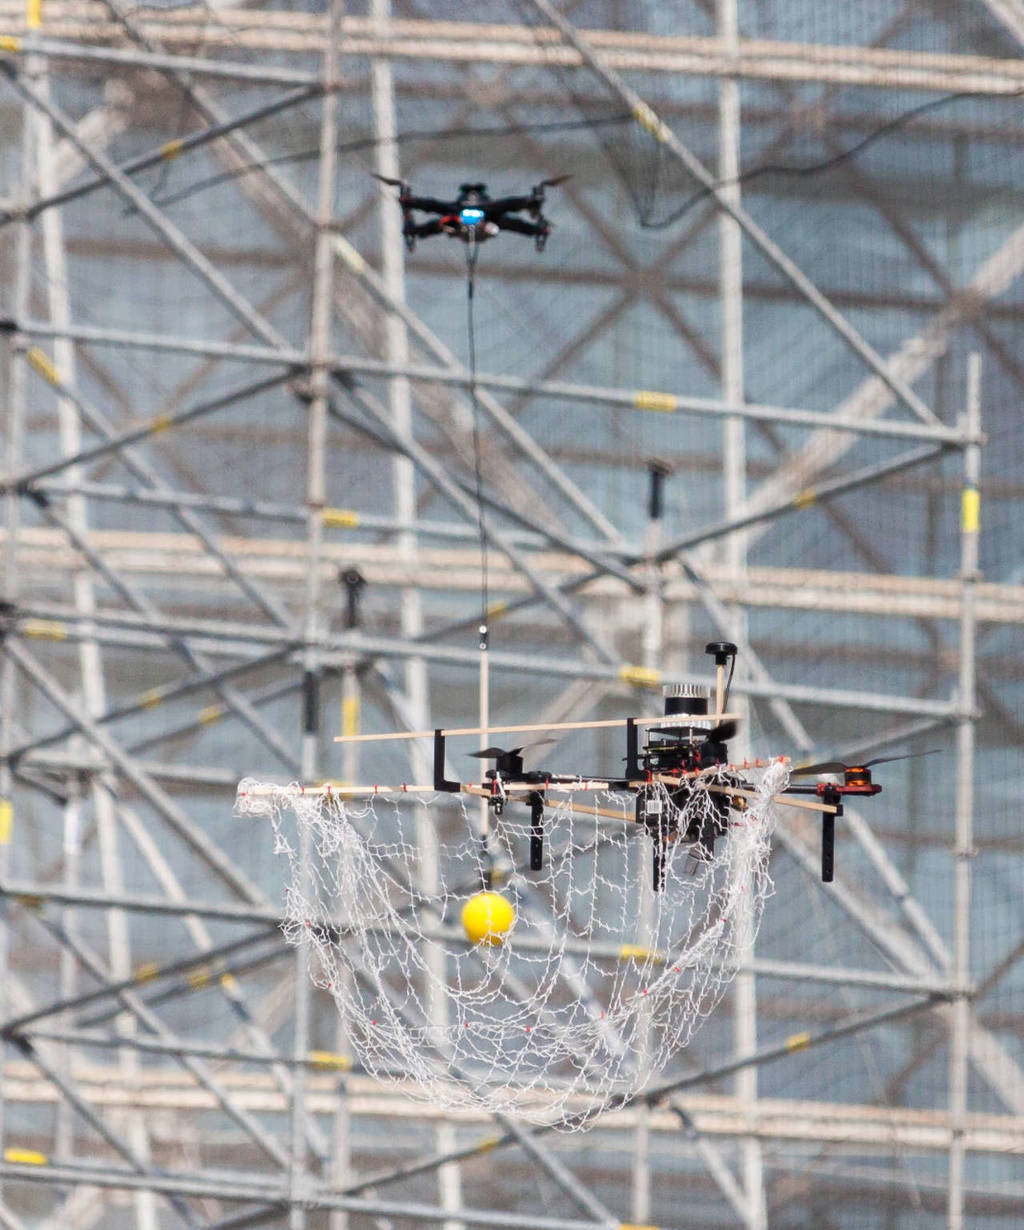
\includegraphics[width=0.155\textwidth]{./fig/photos/ball_catching_1-25_1-5.jpg}};
      \begin{scope}[x={(a.south east)},y={(a.north west)}]
        %%{ grid
        % % useful grid to help you find coordinates for plotting the overlay
        % \draw[black, xstep=.1, ystep=.1] (0,0) grid (1,1);
        % \foreach \i in {0,0.1,0.2,0.3,0.4,0.5,0.6,0.7,0.8,0.9,1} {
        %   \node[align=center] at (\i, -0.05) {\i};
        %   \node[align=center] at (\i, 1.05) {\i};
        %   \node[align=center] at (-0.05, \i) {\i};
        %   \node[align=center] at (1.05, \i) {\i};
        % }
        %%}
        % plot some stuff over the image
        \fill[white] (0.001, 0.001) rectangle (0.18,0.13);
        \fill[draw=black, draw opacity=0.5, fill opacity=0] (0,0) rectangle (1, 1);
        \draw (0.09,0.06) node [text=black] {\small (b)};
      \end{scope}
    \end{tikzpicture}}
    \hfill%
    \subfloat {\begin{tikzpicture}
      \node[anchor=south west,inner sep=0] (a) at (0,0) { 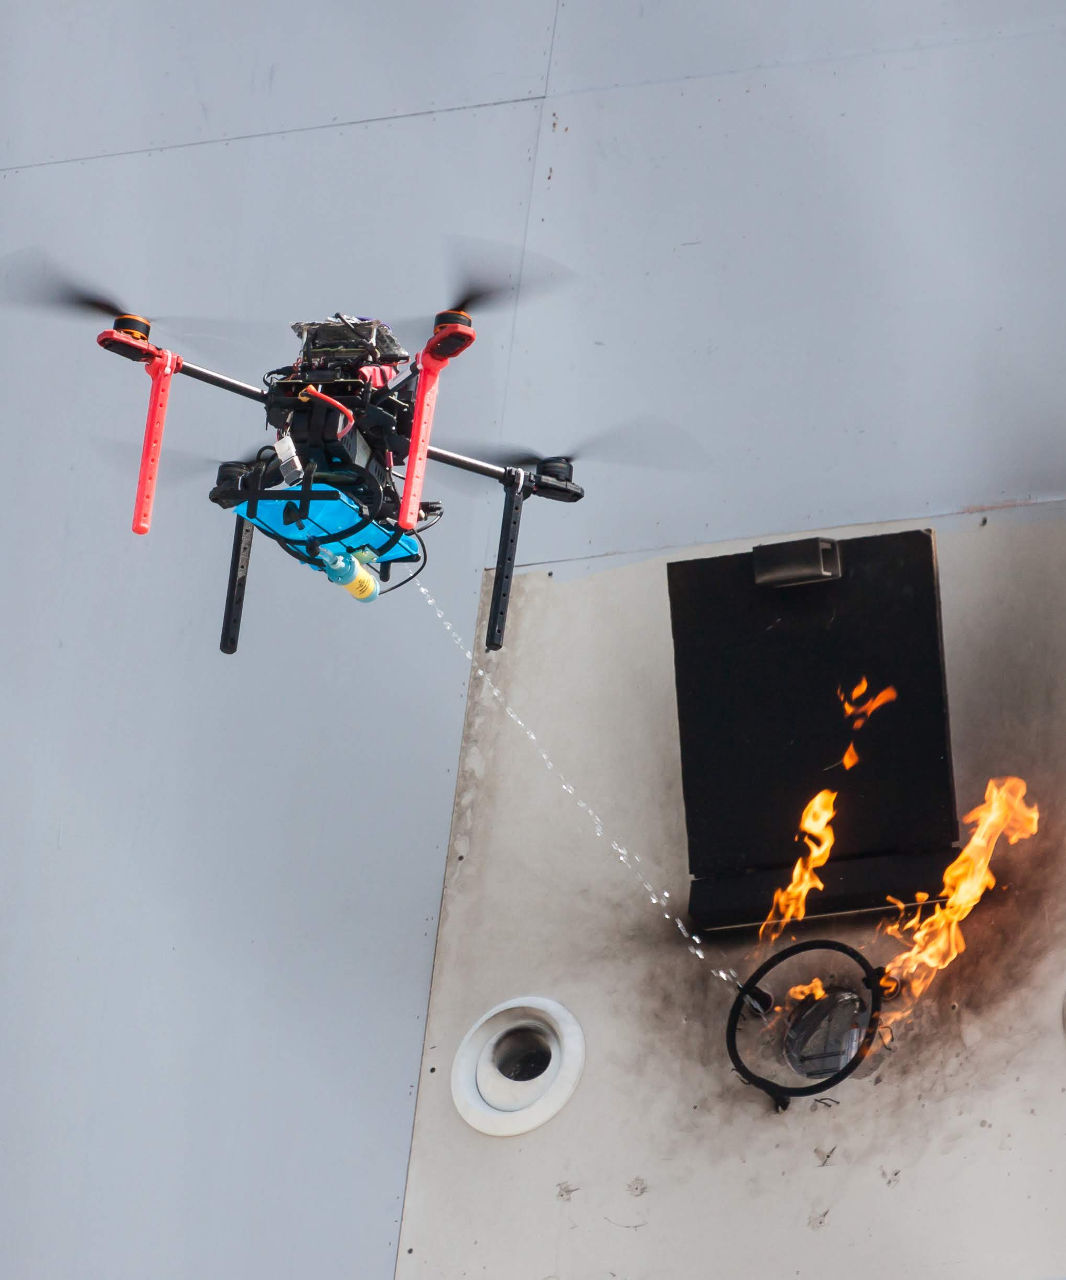
\includegraphics[width=0.155\textwidth]{./fig/photos/ext_1-25_1-5.jpg}};
      \begin{scope}[x={(a.south east)},y={(a.north west)}]
        %%{ grid
        % % useful grid to help you find coordinates for plotting the overlay
        % \draw[black, xstep=.1, ystep=.1] (0,0) grid (1,1);
        % \foreach \i in {0,0.1,0.2,0.3,0.4,0.5,0.6,0.7,0.8,0.9,1} {
        %   \node[align=center] at (\i, -0.05) {\i};
        %   \node[align=center] at (\i, 1.05) {\i};
        %   \node[align=center] at (-0.05, \i) {\i};
        %   \node[align=center] at (1.05, \i) {\i};
        % }
        %%}
        % plot some stuff over the image
        \fill[white] (0.001, 0.001) rectangle (0.18,0.13);
        \fill[draw=black, draw opacity=0.5, fill opacity=0] (0,0) rectangle (1, 1);
        \draw (0.09,0.06) node [text=black] {\small (c)};
      \end{scope}
    \end{tikzpicture}}\\
    \vspace{-0.8em}
    \subfloat {\begin{tikzpicture}
      \node[anchor=south west,inner sep=0] (a) at (0,0) { 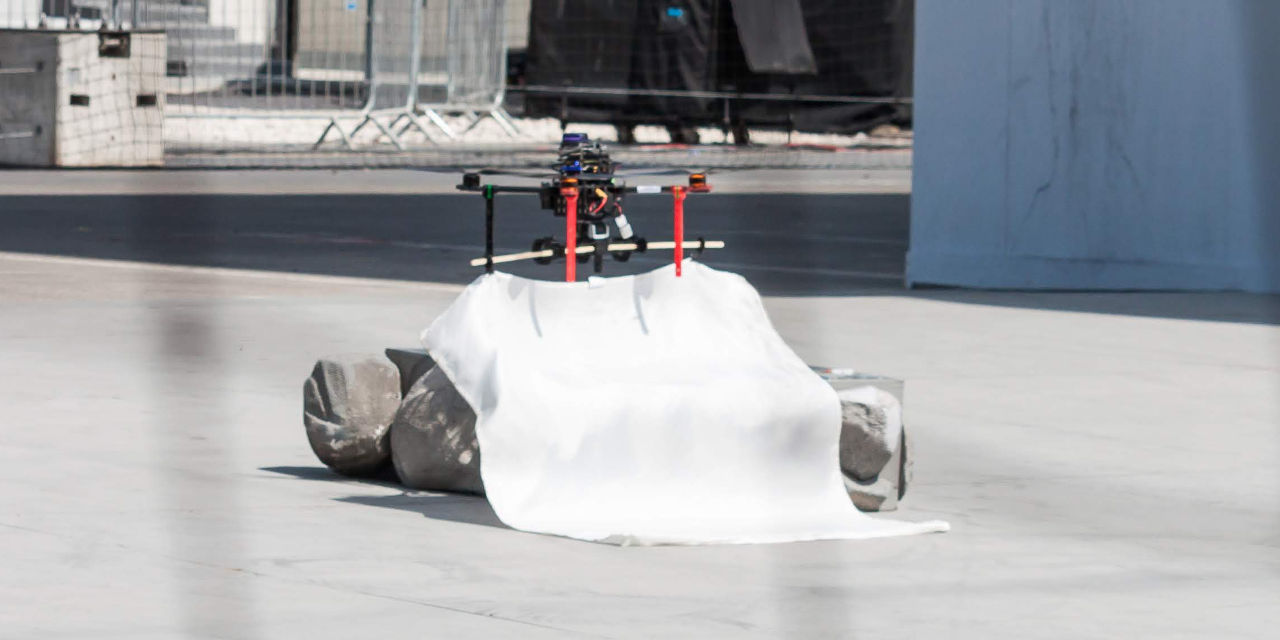
\includegraphics[width=0.235\textwidth]{./fig/photos/blanket_2_1.jpg}};
      \begin{scope}[x={(a.south east)},y={(a.north west)}]
        %%{ grid
        % % useful grid to help you find coordinates for plotting the overlay
        % \draw[black, xstep=.1, ystep=.1] (0,0) grid (1,1);
        % \foreach \i in {0,0.1,0.2,0.3,0.4,0.5,0.6,0.7,0.8,0.9,1} {
        %   \node[align=center] at (\i, -0.05) {\i};
        %   \node[align=center] at (\i, 1.05) {\i};
        %   \node[align=center] at (-0.05, \i) {\i};
        %   \node[align=center] at (1.05, \i) {\i};
        % }
        %%}
        % plot some stuff over the image
        \fill[white] (0.001, 0.001) rectangle (0.13,0.20);
        \fill[draw=black, draw opacity=0.5, fill opacity=0] (0,0) rectangle (1, 1);
        \draw (0.065,0.090) node [text=black] {\small (d)};
      \end{scope}
    \end{tikzpicture}}
    \hfill%
    \subfloat {\begin{tikzpicture}
      \node[anchor=south west,inner sep=0] (a) at (0,0) { 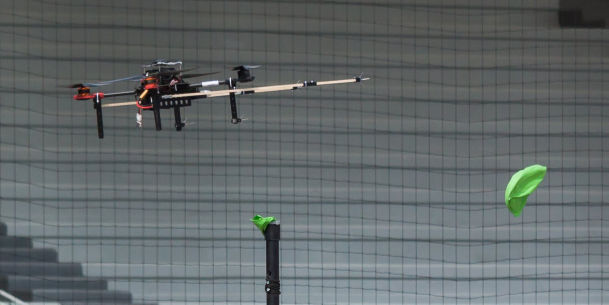
\includegraphics[width=0.235\textwidth]{./fig/photos/popping_2_1.jpg}};
      \begin{scope}[x={(a.south east)},y={(a.north west)}]
        %%{ grid
        % % useful grid to help you find coordinates for plotting the overlay
        % \draw[black, xstep=.1, ystep=.1] (0,0) grid (1,1);
        % \foreach \i in {0,0.1,0.2,0.3,0.4,0.5,0.6,0.7,0.8,0.9,1} {
        %   \node[align=center] at (\i, -0.05) {\i};
        %   \node[align=center] at (\i, 1.05) {\i};
        %   \node[align=center] at (-0.05, \i) {\i};
        %   \node[align=center] at (1.05, \i) {\i};
        % }
        %%}
        % plot some stuff over the image
        \fill[white] (0.001, 0.001) rectangle (0.13,0.20);
        \fill[draw=black, draw opacity=0.5, fill opacity=0] (0,0) rectangle (1, 1);
        \draw (0.065,0.090) node [text=black] {\small (e)};
      \end{scope}
    \end{tikzpicture}}
    \caption{The CTU-UPENN-NYU team during the MBZIRC 2020 competition. The photos depict (a) autonomous wall building, (b) autonomous ball catching, (c) autonomous fire extinguishing, (d) autonomous fire blanket deployment, and (e) autonomous balloon popping.}
    \label{fig:mbzirc_2020}
  \end{figure}

  \subsection{IEEE RAS Summer School on Multi-robot Systems}

  The proposed system was used as an educational tool during the 2019 \ac{IEEE} \ac{RAS} summer school on multirobot systems\footnote{\url{http://mrs.felk.cvut.cz/summer-school-2019}}.
  More than 70 international students were challenged to solve a multi-UAV Dubins traveling salesman problem with neighborhoods during the summer school exercises.
  Student solutions were put to test during an outdoor experimental session.

  %\begin{figure}
  %  \centering
  %  \subfloat {\begin{tikzpicture}
  %    \node[anchor=south west,inner sep=0] (a) at (0,0) { 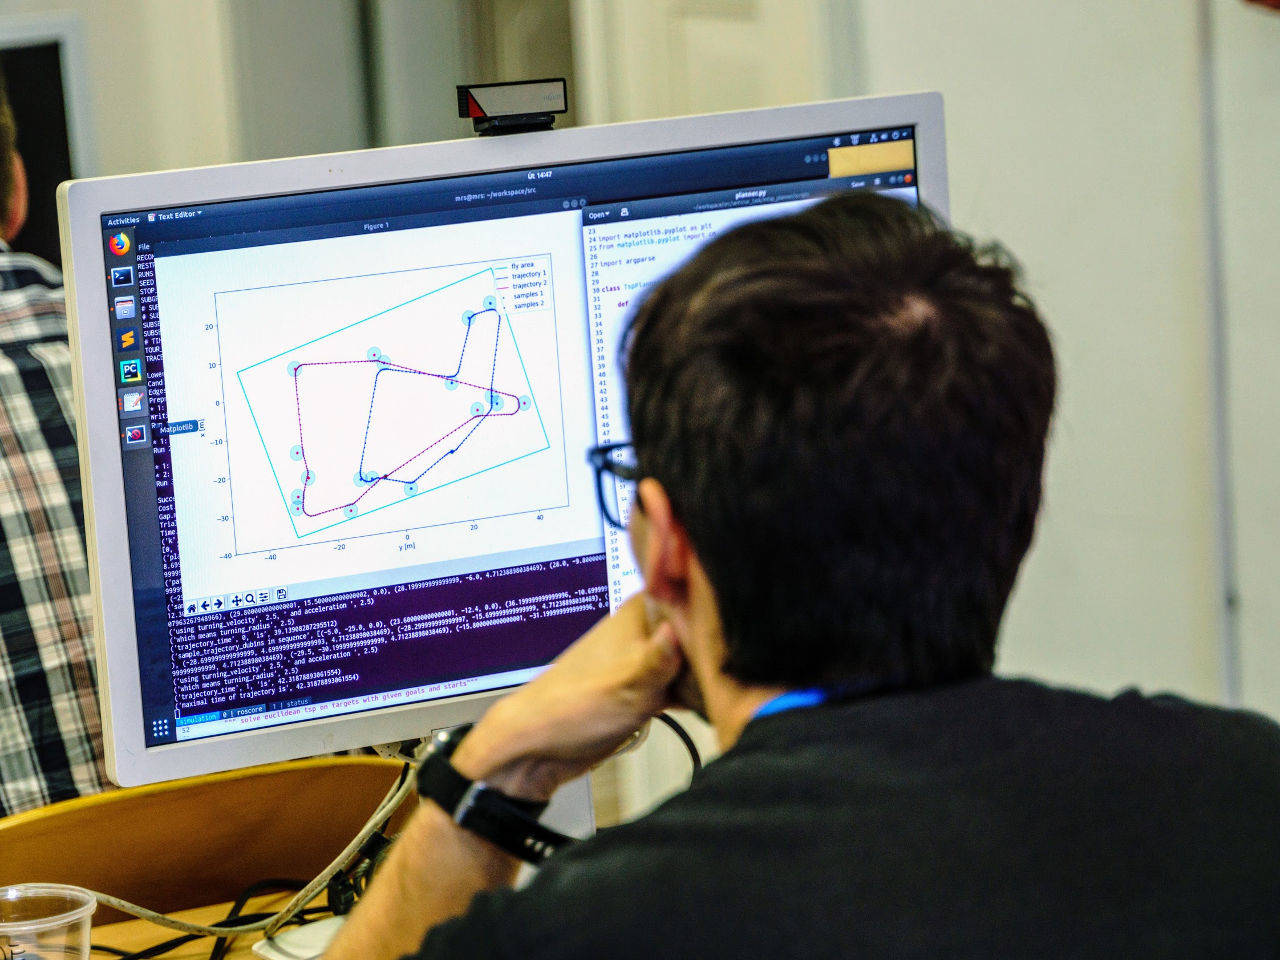
\includegraphics[width=0.235\textwidth]{./fig/photos/summer_schoo_pc.jpg}};
  %    \begin{scope}[x={(a.south east)},y={(a.north west)}]
  %      %%{ grid
  %      % % useful grid to help you find coordinates for plotting the overlay
  %      % \draw[black, xstep=.1, ystep=.1] (0,0) grid (1,1);
  %      % \foreach \i in {0,0.1,0.2,0.3,0.4,0.5,0.6,0.7,0.8,0.9,1} {
  %      %   \node[align=center] at (\i, -0.05) {\i};
  %      %   \node[align=center] at (\i, 1.05) {\i};
  %      %   \node[align=center] at (-0.05, \i) {\i};
  %      %   \node[align=center] at (1.05, \i) {\i};
  %      % }
  %      %%}
  %      % plot some stuff over the image
  %      \fill[white] (0.001, 0.001) rectangle (0.12,0.13);
  %      \fill[draw=black, draw opacity=0.5, fill opacity=0] (0,0) rectangle (1, 1);
  %      \draw (0.06,0.06) node [text=black] {\small (a)};
  %    \end{scope}
  %  \end{tikzpicture}}
  %  \hfill%
  %  \subfloat {\begin{tikzpicture}
  %    \node[anchor=south west,inner sep=0] (a) at (0,0) { 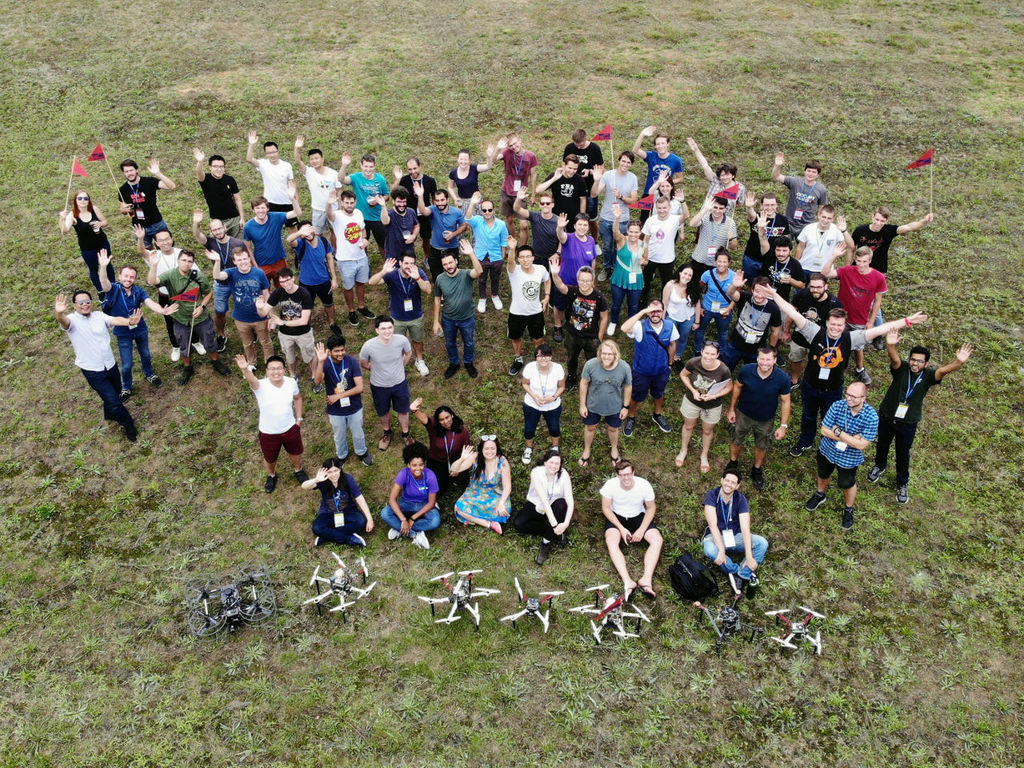
\includegraphics[width=0.235\textwidth]{./fig/photos/summer_school_outdoor.jpg}};
  %    \begin{scope}[x={(a.south east)},y={(a.north west)}]
  %      %%{ grid
  %      % % useful grid to help you find coordinates for plotting the overlay
  %      % \draw[black, xstep=.1, ystep=.1] (0,0) grid (1,1);
  %      % \foreach \i in {0,0.1,0.2,0.3,0.4,0.5,0.6,0.7,0.8,0.9,1} {
  %      %   \node[align=center] at (\i, -0.05) {\i};
  %      %   \node[align=center] at (\i, 1.05) {\i};
  %      %   \node[align=center] at (-0.05, \i) {\i};
  %      %   \node[align=center] at (1.05, \i) {\i};
  %      % }
  %      %%}
  %      % plot some stuff over the image
  %      \fill[white] (0.001, 0.001) rectangle (0.12,0.13);
  %      \fill[draw=black, draw opacity=0.5, fill opacity=0] (0,0) rectangle (1, 1);
  %      \draw (0.06,0.06) node [text=black] {\small (b)};
  %    \end{scope}
  %  \end{tikzpicture}}
  %  \caption{The 2019 IEEE RAS summer school on multirobot systems organized theoretical lectures, (a) exercises with the proposed system, and (b) a practical experimental session, in which students competed in an automatic planning challenge. Go to \protect\url{http://youtu.be/m_AxZs-_DXI} for a summary video from the event.}
  %  \label{fig:summer_school_2019}
  %\end{figure}

%%}

%% | ------------------------ Chapter 5 ----------------------- |

%%{ Ionizing Radiation Detection and Localization by UAVs

\chapternoclear{Ionizing Radiation Detection and Localization by UAVs}
\chaptermark{Ionizing Radiation Localization}

Ongoing research realized in the accepted TACR 2020-2022 project FW01010317:\\
``\textit{Lokalizace zdrojů ionizující radiace pomocí malých bezpilotních helikoptér s detektorem na principu Comptonovy kamery}''.

Relevant author's publications (will be discussed):
\fullciteinbox{baca2016miniaturized}{}
\fullciteinbox{baca2018timepix}{}

Author's publications to be included in the thesis:
\includepaper{baca2018rospix}
\includepaper{baca2019timepix}
\includepaper{stibinger2020localization}

Related author's publications: \cite{baca2016miniaturized, urban2017vzlusat}

\section{Compton $\gamma$-ray camera}

Partially published in \cite{baca2019timepix}, no need to describe extensively.

\section{Monte-Carlo camera model}

Work-in-progress, will describe the principles and publish the simulations.

\section{Radiation source localization and state estimation}

Work-in-progress, will describe the principles and publish the simulations.

%%}

%% | ------------------------ Chapter 6 ----------------------- |

%%{ Conclusion

\chapternoclear{Conclusion}

%%}

%%{ References

\appendix
\renewcommand\chaptername{Appendix}

\chapternoclear{References}

Below are listed all publications of the author.
Each citation is displayed with percentage contribution of the author and number of citations based on Web of Science~(WoS), Scopus and Google Scholar~(GS).
\todo{updated citations}
% Journal articles also contains information about the Impact Factor~(IF) by Web of Science and the CiteScore~(CS) by Scopus.
% The publications~\cite{loianno2018localization, petrlik2020robust, stibinger2020localization, saikin2020wildfire} are only reported with CS due to the novelty of the journal that is expected to receive impact factor in June 2020.

\section{Thesis-related author's publications}

\subsection*{Thesis-related articles in peer-reviewed journals with Impact Factor~(IF)}
\printbibliography[keyword={mine},keyword={phd_related},keyword={journal},keyword={if},heading=none,title={}]

\subsection*{Thesis-related articles --- submitted}
\printbibliography[keyword={mine},keyword={phd_related},keyword={journal},keyword={submitted},heading=none,title={}]

% \subsection*{Thesis-related articles in peer-reviewed journals only with CiteScore~(CS)}
% \printbibliography[keyword={mine},keyword={phd_related},keyword={journal},keyword={cs},heading=none,title={}]

\subsection*{Thesis-related conference proceedings}
\printbibliography[keyword={mine},keyword={phd_related},keyword={conference},heading=none,title={}]

\section{Partially-related author's publications}

\subsection*{Articles in peer-reviewed journals with Impact Factor~(IF)}
\printbibliography[keyword={mine},keyword={phd_unrelated},keyword={journal},keyword={if},heading=none,title={}]

\subsection*{Conference proceedings}
\printbibliography[keyword={mine},keyword={phd_unrelated},keyword={conference},heading=none,title={}]

\section{Cited references}
\printbibliography[notkeyword=mine,heading=none,title={}]

%%}

%%{ Apendices

\appendix
\renewcommand\chaptername{Citations of author's publications}

\chapternoclear{Citations of author's publications}

Below are listed all citations of author's publications without self-citations.

\DeclareCiteCommand{\fullcite}
{\usebibmacro{prenote}}
{\clearfield{addendum}%
  \usedriver
  {\defcounter{minnames}{6}%
  \defcounter{maxnames}{6}}
{\thefield{entrytype}}}
{\multicitedelim}
{\usebibmacro{postnote}}

\noindent
\fullcite{saska2017system}
\begin{refsection}[citations/no_autocit/saska2017system.bib]
  \nocite{*}
  \printbibliography[heading=none,title={},env=favoritebib]
\end{refsection}

% \noindent
% \fullcite{faigl2017onsolution}
% \begin{refsection}[citations/no_autocit/faigl2017onsolution.bib]
%   \nocite{*}
%   \printbibliography[heading=none,title={},env=favoritebib]
% \end{refsection}

% \noindent
% \fullcite{saska2016formations}
% \begin{refsection}[citations/no_autocit/saska2016formations.bib]
%   \nocite{*}
%   \printbibliography[heading=none,title={},env=favoritebib]
% \end{refsection}

\noindent
\fullcite{baca2016miniaturized}
\begin{refsection}[citations/no_autocit/baca2016miniaturized.bib]
  \nocite{*}
  \printbibliography[heading=none,title={},env=favoritebib]
\end{refsection}

\noindent
\fullcite{loianno2018localization}
\begin{refsection}[citations/no_autocit/loianno2018localization.bib]
  \nocite{*}
  \printbibliography[heading=none,title={},env=favoritebib]
\end{refsection}

\noindent
\fullcite{spurny2019cooperative}
\begin{refsection}[citations/no_autocit/spurny2019cooperative.bib]
  \nocite{*}
  \printbibliography[heading=none,title={},env=favoritebib]
\end{refsection}

\noindent
\fullcite{daniel2016terrestrial}
\begin{refsection}[citations/no_autocit/daniel2016terrestrial.bib]
  \nocite{*}
  \printbibliography[heading=none,title={},env=favoritebib]
\end{refsection}

\noindent
\fullcite{baca2017autonomous}
\begin{refsection}[citations/no_autocit/baca2017autonomous.bib]
  \nocite{*}
  \printbibliography[heading=none,title={},env=favoritebib]
\end{refsection}

\noindent
\fullcite{baca2018model}
\begin{refsection}[citations/no_autocit/baca2018model.bib]
  \nocite{*}
  \printbibliography[heading=none,title={},env=favoritebib]
\end{refsection}

\noindent
\fullcite{daniel2017xray}
\begin{refsection}[citations/no_autocit/daniel2017xray.bib]
  \nocite{*}
  \printbibliography[heading=none,title={},env=favoritebib]
\end{refsection}

\noindent
\fullcite{urban2017vzlusat}
\begin{refsection}[citations/no_autocit/urban2017vzlusat.bib]
  \nocite{*}
  \printbibliography[heading=none,title={},env=favoritebib]
\end{refsection}

\noindent
\fullcite{baca2016embedded}
\begin{refsection}[citations/no_autocit/baca2016embedded.bib]
  \nocite{*}
  \printbibliography[heading=none,title={},env=favoritebib]
\end{refsection}

\noindent
\fullcite{baca2019autonomous}
\begin{refsection}[citations/no_autocit/baca2019autonomous.bib]
  \nocite{*}
  \printbibliography[heading=none,title={},env=favoritebib]
\end{refsection}

\noindent
\fullcite{saska2017documentation}
\begin{refsection}[citations/no_autocit/saska2017documentation.bib]
\nocite{*}
\printbibliography[heading=none,title={},env=favoritebib]
\end{refsection}

\noindent
\fullcite{giernacky2019realtime}
\begin{refsection}[citations/no_autocit/giernacky2019realtime.bib]
  \nocite{*}
  \printbibliography[heading=none,title={},env=favoritebib]
\end{refsection}

\noindent
\fullcite{chudoba2014localization}
\begin{refsection}[citations/no_autocit/chudoba2014localization.bib]
  \nocite{*}
  \printbibliography[heading=none,title={},env=favoritebib]
\end{refsection}

\noindent
\fullcite{saikin2020wildfire}
\begin{refsection}[citations/no_autocit/saikin2020wildfire.bib]
  \nocite{*}
  \printbibliography[heading=none,title={},env=favoritebib]
\end{refsection}

\noindent
\fullcite{daniel2019inorbit}
\begin{refsection}[citations/no_autocit/daniel2019inorbit.bib]
  \nocite{*}
  \printbibliography[heading=none,title={},env=favoritebib]
\end{refsection}

\noindent
\fullcite{baca2018timepix}
\begin{refsection}[citations/no_autocit/baca2018timepix.bib]
  \nocite{*}
  \printbibliography[heading=none,title={},env=favoritebib]
\end{refsection}

\noindent
\fullcite{baca2018rospix}
\begin{refsection}[citations/no_autocit/baca2018rospix.bib]
  \nocite{*}
  \printbibliography[heading=none,title={},env=favoritebib]
\end{refsection}

\noindent
\fullcite{spurny2016complex}
\begin{refsection}[citations/no_autocit/spurny2016complex.bib]
  \nocite{*}
  \printbibliography[heading=none,title={},env=favoritebib]
\end{refsection}

\noindent
\fullcite{chudoba2016exploration}
\begin{refsection}[citations/no_autocit/chudoba2016exploration.bib]
  \nocite{*}
  \printbibliography[heading=none,title={},env=favoritebib]
\end{refsection}

%%}

\end{document}
